\documentclass[oneside,12pt]{book}

% e-book format
\usepackage[paperwidth=210mm,paperheight=148mm,margin=10mm]{geometry}

% Cyrillization
\usepackage[T1,T2A]{fontenc}
\usepackage[utf8]{inputenc}
\usepackage[english,russian]{babel}
\usepackage{indentfirst}

% font setup for screen reading
\renewcommand{\familydefault}{\sfdefault}
\normalfont

% pdflatex options
\usepackage[unicode,colorlinks,linkcolor=blue,bookmarks=true]{hyperref}
\usepackage[pdftex]{graphicx}

% listings
\usepackage{verbatim}
\usepackage{listings}
\lstset{
extendedchars=true,inputencoding=utf8, % i18n
frame=single, % show frames around
numbers=left, numberstyle=\small,numbersep=1mm,% line numbering
tabsize=4, % tab style
% keywordstyle=\color{blue}\texttt,
% commentstyle=\color{magenta}\texttt,
% showspaces=false
}
\newcommand{\lst}[3]{\lstinputlisting[title=\href{#2}{#1}]{#3}}

% software menu & keys
\usepackage[os=win]{menukeys} 
\usepackage{amssymb} % windows key
\newcommand{\winstart}{$\boxplus$}
\newcommand{\winr}{\keys{\winstart+R}}
\newcommand{\file}[1]{\textbf{\textsf{#1}}}
\newcommand{\lms}{$\lhd$}
\newcommand{\dblms}{$\lhd\lhd$}
\newcommand{\rms}{$\rhd$}
\newcommand{\checkbox}{$\boxtimes$}
\newcommand{\uncheckbox}{$\square$}

% disable oneliner page breaks
\usepackage[defaultlines=2,all]{nowidow}

% books bib management
\usepackage{biblatex}
\addbibresource{../bib/python.bib}
\addbibresource{../bib/eskd.bib}
\addbibresource{../bib/electronics.bib}
\addbibresource{../bib/latex.bib}
\addbibresource{../bib/sat.bib}


% extra char sets
\usepackage{wasysym} % smileys

% set lists style
% \usepackage{enumitem}
% \setlist{nosep}

% misc

% \usepackage{titling}

\newcommand{\email}[1]{$<$\href{mailto:#1}{#1}$>$}
\newcommand{\internet}{Internet}

\newcommand{\cm}[1]{Cortex-M#1}
\newcommand{\cmx}{\cm{x}}

\newcommand{\linux}{Linux}
\newcommand{\emlinux}{em\linux}

\newcommand{\cpp}{$C^{+}_{+}$}
\newcommand{\py}{Python}

\newcommand{\vcs}{\hyperref[vcs]{VCS}}
\newcommand{\make}{\hyperref[make]{Make}}
\newcommand{\spice}{ngSPICE}
\newcommand{\latex}{\LaTeX}

\newcommand{\eclipse}{\textcircled{$\equiv$}\textsc{eclipse}}
\newcommand{\vim}{(g)Vim}

\newcommand{\note}[1]{\footnote{\ #1}}
\newcommand{\cp}[1]{\note{копипаста \url{#1}}}

\newcommand{\win}{\winstart Windows}

\newcommand{\mk}{МК}

\newcommand{\term}[1]{\emph{#1}}

\newcommand{\pref}[1]{/стр.\pageref{#1}/}

% math
\usepackage{cancel}

% titles

\hypersetup{
	pdftitle={Азбука халтурщика-ARMатурщика},
	pdfauthor={ruOpenWrt, HackSpace <<Чебураторный завод>>, Консорциум хоббитов
	России, Bill Collis (Часть 1)}, 
	pdfsubject={https://github.com/ponyatov/Azbuka}
}


\begin{document}

\begin{titlepage}

\noindent
\includegraphics[height=0.4\textheight]{logo/CHBZ.png}
\hspace{1cm}
\includegraphics[height=0.15\textheight]{logo/LinuxPowered.png}
\hspace{1cm}
\includegraphics[height=0.4\textheight]{logo/OpenHardware.png}

\begin{centering}

\begin{framed}
\begin{framed}
{\Huge \textbf{Азбука ARMатурщика}}
\end{framed}

{\large \textsc{основы бытовой автоматики, электроники и систем управления}}
\end{framed}

\end{centering}

\bigskip
\begin{tabular}{p{1cm} l}
{\Large \copyright}
& Консорциум хоббитов России \\
& HackSpace
<<\href{https://github.com/ponyatov/CHBZ/raw/master/presentation.pdf}{Чебураторный
завод}>> \\
& Дмитрий Понятов \email{dponyatov@gmail.com} \\
& группа \href{https://groups.google.com/forum/\#!forum/openwrt2ru}{ruOpenWrt}\\
& Bill Collis (\ref{bcollis}) \\
& Andreas Fester (\ref{spice})\\
& Joe Martin, Craig Libuse (\ref{tabletop}) \\
\end{tabular}

\end{titlepage}


\tableofcontents

Linux для встраиваемых систем\note{будем называть его \emlinux}\ ---
популярный метод быстрого создания комплекса ПО для больших сложных приложений,
работающих на достаточно мощном железе, особенно предполагающих интенсивное
использование сетевых технологий.

За счет использования уже существующей и очень большой базы исходных текстов
ядра, библиотек и программ для \linux, бесплатно доступных в т.ч. и для
коммерческих приложений, можно на порядки сократить стоимость разработки
собственных программных компонентов, и при этом получить готовую команду
бесплатных стронних разработчиков, уже знакомых с созданием ПО для \linux.

Из недостатков можно отметить:
\begin{itemize}
  \item Отсутствие полноценной поддержки режима жесткого реального времени;
  \item Тяжелое ядро;
  \begin{itemize}
  \item Поддерживаются только мощные семейства процессоров\note{32-бит,
  необходим блок MMU};
  \item Значительные требования по объему \ram\ и общей производительности;
  \end{itemize}
  \item Дремучесть техспециалистов, контуженных ТурбоПаскалем и
Win\-dows\-ом;
\end{itemize}

Для \term{сборки}\ \emlinux-системы используется метод \term{кросс-компиляции},
когда используется \term{кросс-тулчейн}, компилирующий весь комплект ПО для
компьютера с другой архитектурой. Типичный пример\ --- сборка ПО на
ПК c процессором Intel i7 для Raspberry Pi или планшета на процессоре
AllWinner/Tegra/\ldots.

\emlinux\ очень широко применяется на рынке мобильных устройств\note{в т.ч.
является основой Android}, и устройств интенсивно использующих сетевые протоколы
(роутеры, медиацентры).

В качествe примера применения рассмотрим относительно простое приложение:
многофункциональные настенные часы с синхронизацией времени через \internet, с
будильником, медиапроигрывателем, блэкджеком и плюшками.


\secrel{Введение в практическую электронику} \label{bcollis}\secdown
\input{bcollis/thanks}
\chapter{1 Введение в практическую электронику 13}

Эта книга\note{оригинал: B.Collis The Introduction to Practical 
Electronics\ldots}\ имеет слеующий ряд основных направлений:

\begin{itemize}
  \item Распознавание электронных компонентов и их правильное использование
  \item Наработка цельного набора компетенций в базовой электронике
  \item Использование макетных плат
  \item Навыки ручной пайки
  \item Использование закона Ома для выбора токоограничивающих резисторов
  \item Делитель напряжения
  \item Использование EDA CAD\note{\keys{E}\,lectronic \keys{D}\,esign
  \keys{A}\,utomation, САПР автоматизации проектирования электроники}\ для
  разработки и подготовки производства печатных плат
  \item Программирование микроконтроллеров и их сопряжение
  \item Транзистор в ключевом режиме
  \item Теория источников питания
  \item Принципы и схемы электропривода
  \item Моделирование решений через тестирование и испытания
  \item Следование кодексу практики
  \item Безопасные приемы работы
\end{itemize}

\section{Ваше обучение по специальности <<Технология>>}

\begin{itemize}

\item \textbf{Технологическая практика}

\begin{itemize}

\item\textbf{Быть четким}: разработка четких спецификаций для ваших
технологических проектов.

\item\textbf{Планирование}: думать прежде чем делать, и использовать во время
работы наброски типа блок-схем, принципиальных схем, чертежей разводки плат,
диаграмм и эскизов.

\item\textbf{Работа на результат}: испытания, тестирование и сборка электронных
схем, проектирование и изготовление печатных плат, написание программ для
микроконтроллеров.

\end{itemize}

\item \textbf{Технологические знания}

\begin{itemize}

\item\textbf{Технологическое моделирование}: прежде чем строить электронное
устройство, важно понять как оно работает сначала путем моделирования и/или
тестирования аппаратного и программного обеспечения.

\item\textbf{Технологические продукты}: знания о компонентах и ​​их
характеристиках.

\item\textbf{Технологические системы}: электронное устройство является более,
чем набором компонентов, это функционирующая система с входами, выходами и
контролирующим процессом.

\end{itemize}

\item \textbf{Природа технологии}

\begin{itemize}

\item\textbf{Характеристики технологических достижений}: знания об электронных
компонентах, особенно микроконтроллерах как основа современных технологий.

\item\textbf{Роль технологии}: электронные устройства в настоящее время играют
центральную роль в инфраструктуре нашего современного общества; мы их хозяева,
как они изменили нашу жизнь?

\end{itemize}

\end{itemize}

\section{Ключевые компетенции Ново-Зеландской программы}

\begin{itemize}

\item\textbf{Размышление}: для меня задачей технологии является все что касается
размышления. Моя цель: заставить студентов понимать технологии, использованные в
электронных устройствах. Для достижения этой цели студенты должны активно
взаимодействовать с их работой на самом раннем этапе, чтобы они могли построить
свое собственное понимание и пойти дальше, чтобы стать хорошими решалами
проблем. В начале своего обучения в электронике это требует от студентов
понимания инструкций, которые им дают и поиск ясности, когда они не понимают их.
Для этого многие новые и различные элементы знаний рассматриваются на занятиях,
и студентам выдаются задания на решение проблем чтобы помочь им мыслить
логически. Копирование чужого ответа является ошибочным, но приветствуется
совместная работа. В основе обучения лежит построение правильных концептуальных
моделей и анализ в контексте "большой картины".

\item\textbf{Relating to others} – working together in pairs and groups is as
essential in the classroom as it is in any other situation in life; we all have to share and negotiate resources and equipment
with others; it is essential therefore to actively communicate with each other and assist one
other.

\item\textbf{Using language symbols and texts} – At the heart of our subject is
the language we use for communicating electronic circuits, concepts, algorithms and computer programming syntax; so
the ability to recognise and using symbols and diagrams correctly for the work we do is vital.

\item\textbf{Managing self} – This is about students taking personal
responsibility for their own learning; it is about challenging students who expect to read answers in a book or have a teacher tell them
what to do. It means that students need to engage with the material in front of them.
Sometimes the answers will come easily, sometimes they will not; often our subject involves a
lot of trial and error (mostly error). Students should know that it is in the tough times that the
most is learnt. And not to give up keep searching for understanding.

\item\textbf{Participating and contributing} – We live in a world that is
incredibly dependent upon technology especially electronics, students need to develop an awareness of the importance
of this area of human creativity to our daily lives and to recognise that our projects have a
social function as well as a technical one.

\end{itemize}


\chapter{2 Вводная электронная схема 15}

\section{2.1 Где купить комплектующие? 15}

В Новой Зеландии есть некоторое количество отличных поставщиков компонентов с
разумными ценами, включающих \url{www.surplustronics.co.nz}, и
\url{www.activecomponents.com}. Зарубежные поставщики, которых я использую,
включают \url{www.digikey.co.nz}, \url{www.sparkfun.com}, \url{ebay.com}
и \url{aliexpress.com}

\bigskip
\includegraphics[width=0.8\textwidth]{bcollis/breadboard2.jpg}

Макетная плата (breadboard)\ --- пластмассовый блок с отверстиями и
металлическими полосковыми металлическими зажимами, создающими соединения между
элементами схемы. Отверстия расположены так, что компоненты могут быть соединены
вместе формируя схему. Верхние и нижние ряды, как правило, используется для шин
питания, красный сверху для плюса, и внизу черный/синий для для минуса (общий
провод).

\includegraphics[width=0.8\textwidth]{bcollis/BreadboardConnections.jpg}

\bigskip

Эта схема \ref{ch21sch}\ может быть собрана вот так \ref{ch21lay}, обратите
внимание, что светодиод должен находиться в правильном положении. Если у вас
есть светодиод и резистор, соединенные в замкнутый контур, светодиод должен
загореться.

\bigskip
Принципиальная схема \label{ch21sch}

\bigskip
Компоновка \label{ch21lay}

\bigskip
The LED requires 2V the battery is 9V, if you put the LED across the battery it
would stop working! So a 1k (1000ohm) resistor is used to reduce the voltage to
the LED and the current through it, get a multimeter and measure the voltage
across the resistor, is it close to 7V? If you disconnect any wire within the
circuit it stops working, a circuit needs to be complete before electrons can
flow.

\section{2.2 Определение сопротивления резистора по цветовому коду 16}

.

\section{2.3 Светодиоды 17}

.

\section{2,4 Некоторые технические характеристики светодиода 17}

.

\section{2.5 Задание на исследование светодиода 17}

.

\section{2.6 Добавление выключателя  в схему 18}

.

\section{2.7 Задание на установку выключателя 18}

.

\section{2,8 Важные понятия схемы 19}

.

\section{2.9 Изменение величины сопротивления 19}

.

\section{2.10 Добавление транзистора в схему 20}

.

\section{2.11 Чтение схем 21}

.

\section{2.12 Входная цепь\ --- LDR 22}

.

\section{2.13 Рабочая схема датчика темноты 23}

.

\section{2,14 Защитные цепи - использование диода 24}

.

\section{2.15 Задача исследования диода 24}

.

\section{2.13 Финальная схема датчика темноты 23}

.



% \chapter{3 Вводное конструирование печатной платы 26}
% % 3.1 Eagle Schematic and Layout Editor Tutorial  26
% % 3.2 An Introduction to Eagle  27
% % 3.3 The Schematic Editor  28
% % 3.4 The Board Editor . 33
% % 3.5 Making Negative Printouts . 37
% % 3.6 PCB Making  38
% 
% \chapter{4 Пайка, припой и паяльники 41}
% % 4.1 Soldering facts . 42
% % 4.2 Soldering Safety  42
% % 4.3 Soldering wires to switches  43
% % 4.4 Codes of practice  44
% % 4.5 Good and bad solder joints  45
% % 4.6 Short circuits . 46
% % 4.7 Soldering wires to LED’s . 48
% \chapter{5 Введение в теорию электроники 49}
% % 5.1 Making electricity  49
% % 5.2 ESD electrostatic discharge  51
% % 5.3 Magnets, wires and motion  52
% % 5.4 Group Power Assignment  52
% % 5.5 Electricity supply in New Zealand  53
% % 5.6 Conductors  54
% % 5.7 Insulators  54
% % 5.8 Choosing the right wire  55
% % 5.9 Resistors . 56
% % 5.10 Resistor Assignment . 56
% % 5.11 Resistivity  56
% % 5.12 Resistor prefixes . 57
% % 5.13 Resistor Values Exercises . 58
% % 5.14 Capacitors  60
% % 5.15 Component symbols reference  61
% % 5.16 Year 10/11 - Typical test questions so far  62
% \chapter{6 Введение в электронику микроконтроллера 63}
% % 6.1 What is a computer? . 64
% % 6.2 What does a computer system do?  64
% % 6.3 What does a microcontroller system do? . 65
% % 6.4 What exactly is a microcontroller?  66
% % 6.5 Getting started with AVR Programming  67
% % 6.6 Breadboard  67
% % 6.7 Breadboard+Prototyping board circuit  68
% % 6.8 Checking your workmanship . 70
% % 6.9 Getting started with Bascom & AVR  71
% % 6.10 The compiler . 71
% % 6.11 The programmer . 71
% % 6.12 USBASP programming cable  72
% % 6.13 Your first circuit  73
% % 6.14 An introduction to flowcharts . 74
% % 6.15 Bascom output commands . 75
% % 6.16 Exercises  76
% % 6.17 Two delays . 77
% % 6.18 Syntax errors -‘bugs’ . 78
% % 6.19 Microcontroller portswrite a Knightrider program using LED’s  79
% % 6.20 Knightrider v2  80
% % 6.21 Knightrider v3  81
% % 6.22 Commenting your programs  83
% % 6.23 Learning review  83
% % 6.24 What is a piezo and how does it make sound?. 84
% % 6.25 Sounding Off . 85
% % 6.26 Sound exercises . 87
% % 6.27 Amp it up . 88
% \chapter{7 Входные цепи микроконтроллера 91}
% % 7.1 Single push button switch  91
% % 7.2 Pullup resistor theory  93
% % 7.3 Switch in a breadboard circuit  93
% % 7.4 Checking switches in your program  94
% % 7.5 Program Logic – the ‘If-Then’ Switch Test  95
% % 7.6 If-then exercises  96
% % 7.7 Switch contact bounce . 97
% % 7.8 Reading multiple switches  99
% % 7.9 Bascom debounce command . 100
% % 7.10 Different types of switches you can use  101
% % 7.11 Reflective opto switch  102
% \chapter{8 Обзор программирования 104}
% % 8.1 Three steps to help you write good programs  104
% % 8.2 Saving Programs . 104
% % 8.3 Organisation is everything  104
% % 8.4 Programming template  105
% % 8.5 What you do when learning to program . 106
% % 8.6 AVR microcontroller hardware  107
% % 8.7 Power supplies 107
% % 8.8 Programming words you need to be able to use correctly  110
% % 8.9 Year10/11 typical test questions so far  111
% \chapter{9 Введение в поток выполнения программы 112}
% % 9.1 Pedestrian crossing lights controller  112
% % 9.2 Pedestrian Crossing Lights schematic  113
% % 9.3 Pedestrian Crossing Lights PCB Layout 114
% % 9.4 Algorithm planning example – pedestrian crossing lights . 115
% % 9.5 Flowchart planning example – pedestrian crossing lights . 116
% % 9.6 Getting started code  117
% % 9.7 Modification exercise for the pedestrian crossing . 117
% % 9.8 Traffic lights program flow  118
% \chapter{10 Вводное программирование: использование подпрограмм 126}
% % 10.1 Sending Morse code  127
% % 10.2 LM386 audio amplifier PCB. 130
% % 10.3 LM386 PCB Layout . 132
% \chapter{11 Вводное программирование: Использование переменных 134}
% % 11.1 Stepping or counting using variables  135
% % 11.2 For-Next  137
% % 11.3 Siren sound - programming using variables  139
% % 11.4 Make a simple siren  141
% % 11.5 Siren exercise  142
% % 11.6 A note about layout of program code . 143
% % 11.7 Using variables for data  144
% % 11.8 Different types of variables  145
% % 11.9 Variables and their uses  146
% % 11.10 Vehicle counter  147
% % 11.11 Rules about variables  148
% % 11.12 Examples of variables in use . 148
% % 11.13 Byte variable limitations  149
% % 11.14 Random Numbers  150
% % 11.15 The Bascom-AVR simulator  151
% % 11.16 Electronic dice project  152
% % 11.17 Programming using variables – dice  152
% % 11.18 Dice layout stage 1 . 153
% % 11.19 Dice layout stage 2 . 154
% % 11.20 Dice Layout final 155
% % 11.21 First Dice Program flowchart . 156
% % 11.22 A note about the Bascom Rnd command  157
% % 11.23 Modified dice . 158
% % 11.24 Modified Knightrider  160
% \chapter{12 Основные дисплеи 161}
% % 12.1 7 segment displays . 161
% % 12.2 Alphanumeric LED displays  172
% \chapter{13 Проект портативного аудиоусилителя на TDA2822M 174}
% % 13.1 Portfolio Assessment Schedule . 175
% % 13.2 Initial One Page Brief . 176
% % 13.3 TDA2822M specifications  177
% % 13.4 Making a PCB for the TDA2822 Amp Project . 178
% % 13.5 Extra PCB making information  182
% % 13.6 Component Forming Codes of Practice. 183
% % 13.7 TDA2811 wiring diagram  184
% % 13.8 SKETCHUP Quick Start Tutorial  185
% % 13.9 Creating reusable components in SketchUp  186
% \chapter{14 Основы логического программирования 187}
% % 14.1 Quiz Game Controller  187
% % 14.2 Quiz game controller system context diagram  188
% % 14.3 Quiz game controller block diagram  188
% % 14.4 Quiz game controller Algorithm . 190
% % 14.5 Quiz game schematic . 191
% % 14.6 Quiz game board veroboard layout . 192
% % 14.7 Quiz Controller flowchart  196
% % 14.8 'Quiz Controller program code 197
% % 14.9 Don’t delay - use logic  199
% \chapter{15 Разработка алгоритма: Система сигнализации 202}
% % 15.1 Simple alarm system – stage 1 . 202
% % 15.2 Alarm System Schematic . 203
% % 15.3 A simple alarm system – stage 2 208
% % 15.4 A simple alarm system – stage 3 209
% % 15.5 A simple alarm system – stage 4 210
% % 15.6 More complex alarm system . 211
% % 15.7 Alarm unit algorithm 5 212
% % 15.8 Alarm 6 algorithm 213
% \chapter{16 Основы теории цепей постоянного тока 215}
% % 16.1 Conventional Current . 215
% % 16.2 Ground  215
% % 16.3 Preferred resistor values  215
% % 16.4 Resistor Tolerances  216
% % 16.5 Combining resistors in series . 216
% % 16.6 Combining resistors in parallel  217
% % 16.7 Resistor Combination Circuits  218
% % 16.8 Multimeters . 219
% % 16.9 Multimeter controls  220
% % 16.10 Choosing correct meter settings  221
% % 16.11 Ohms law  222
% % 16.12 Voltage & Current Measurements  223
% % 16.14 Continuity  224
% % 16.15 Variable Resistors  225
% % 16.16 Capacitors  226
% % 16.17 Capacitor Codes and Values . 226
% % 16.18 Converting Capacitor Values uF, nF , pF  226
% % 16.19 Capacitor action in DC circuits . 227
% % 16.20 The Voltage Divider  228
% % 16.21 Using semiconductors  229
% % 16.22 Calculating current limit resistors for an LED . 230
% % 16.23 The Bipolar Junction Transistor  231
% % 16.24 Transistor Specifications Assignment  232
% % 16.25 Transistor Case styles  232
% % 16.26 Transistor amplifier in a microcontroller circuit  232
% % 16.27 Transistor Audio Amplifier  233
% % 16.28 Speakers . 234
% % 16.29 Switch types and symbols  235
% \chapter{17 Основы планирования проекта 236}
% % 17.1 System Designer  237
% % 17.2 Project mind map . 241
% % 17.3 Project timeline . 243
% % 17.4 System context diagram  245
% % 17.5 Block Diagram 256
% % 17.6 Board Layouts  258
% % 17.7 Algorithm design  263
% % 17.8 Flowcharts  265
% \chapter{18 Пример дизайна системы: Таймер клеевого пистолета 268}
% % 18.1 System context diagram  268
% % 18.2 Hot glue gun timer block diagram . 269
% % 18.3 Hot glue gun timer algorithm . 270
% % 18.4 Hot glue gun timer flowchart  271
% % 18.5 Hot glue gun timer program. 272
% \chapter{19 Основные интерфейсы и их программирование 273}
% % 19.1 Parallel data communications  274
% % 19.2 LCDs (liquid crystal displays) . 275
% % 19.3 Alphanumeric LCDs  276
% % 19.4 ATTINY461 Development PCB with LCD . 277
% % 19.5 Completing the wiring for the LCD 279
% % 19.6 LCD Contrast Control  280
% % 19.7 Learning to use the LCD  281
% % 19.8 Repetition again - the ‘For-Next’ and the LCD  282
% % 19.9 LCD Exerises . 283
% % 19.10 Defining your own LCD characters . 286
% % 19.11 LCD custom character program  286
% % 19.12 A simple digital clock . 288
% % 19.13 Adding more interfaces to the ATTiny461 Development board . 290
% % 19.14 Ohms law in action – a multicoloured LED . 292
% \chapter{20 Основы интерфейса аналого-цифрового преобразования 295}
% % 20.1 ADC - Analog to Digital conversion . 295
% % 20.2 Light level sensing  295
% % 20.3 Voltage dividers review . 296
% % 20.4 AVR ADC connections  296
% % 20.5 Select-Case  297
% % 20.6 Reading an LDR’s values . 299
% % 20.7 Marcus’ year10 night light project . 301
% % 20.8 Temperature measurement using the LM35  304
% % 20.9 A simple temperature display . 305
% % 20.10 LM35 temperature display  309
% % 20.11 Force Sensitive Resistors  312
% % 20.12 Piezo sensor . 312
% % 20.13 Multiple switches and ADC . 313
% \chapter{21 Основы проектирования системы 314}
% % 21.1 Understanding how systems are put together  314
% % 21.2 Food Processor system block diagram . 314
% % 21.3 Subsystems  314
% % 21.4 Food Processor system functional attributes - algorithm  314
% % 21.5 Food Processor system flowchart  315
% % 21.6 Toaster Design 316
% % 21.7 Toaster - system block diagram  316
% % 21.8 Toaster Algortihm . 316
% \chapter{22 Основы проектирования системы: Тайм-трекер 317}
% % 22.1 System context diagram and brief  318
% % 22.2 Time tracker block diagram . 319
% % 22.3 Algorithm development . 320
% % 22.4 Schematic  320
% % 22.5 Time tracker flowchart and program version 1 321
% % 22.6 Time Tracker stage 2 . 322
% % 22.7 Time Tracker stage 3 . 324
% % 22.8 Time Tracker stage 4 . 326
% \chapter{23 Основы вычислений времени 330}
% % 23.1 Ohms law calculator  330
% % 23.2 more maths - multiplication . 335
% % 23.3 Algorithms for multiplication of very large numbers . 337
% % 23.4 Program ideas - algorithm and flowchart exercises . 339
% \chapter{24 Основы строковых переменных 340}
% % 24.1 Strings assignment . 342
% % 24.2 ASCII Assignment  344
% % 24.3 Time in a string . 347
% % 24.4 Date in a string  349
% % 24.5 Scrolling message assignment  351
% % 24.6 Some LCD programming exercises.  352
% \chapter{25 Cиловые интерфейсы 353}
% % 25.1 Microcontroller power limitations  353
% % 25.2 Power  355
% % 25.3 Power dissipation in resistors . 355
% % 25.4 Diode characteristics  356
% % 25.5 Using Zener diodes . 357
% % 25.6 How diodes work  358
% % 25.7 How does a LED give off light? . 359
% % 25.8 LCD Backlight Data . 360
% % 25.9 Transistors as power switches  361
% % 25.10 High power loads  362
% % 25.11 AVR Power matters  362
% % 25.12 Darlington transistors - high power . 364
% % 25.13 ULN2803 Octal Darlington Driver  366
% % 25.14 Connecting a FET backlight control to your microcontroller  368
% % 25.15 FET backlight control  369
% \chapter{26 Теория источников питания 370}
% % 26.1 Typical PSUs . 371
% % 26.2 The four stages of a PSU (power supply unit)  372
% % 26.3 Stage 1step down transformer  372
% % 26.4 Stage 2AC to DC Conversion  374
% % 26.5 Stage 3Filtering AC component . 375
% % 26.6 Stage 4Voltage Regulation  375
% % 26.7 Ripple (decibel & dB) . 379
% % 26.8 Line Regulation . 380
% % 26.9 Load Regulation  380
% % 26.10 Current Limit . 381
% % 26.11 Power, temperature and heatsinking . 384
% % 26.12 Typical PSU circuit designs  386
% % 26.13 PSU block diagram  386
% % 26.14 PSU Schematic  386
% % 26.15 Practical current limit circuit.  389
% % 26.16 Voltage measurement using a voltage divider  391
% % 26.17 Variable power supply voltmeter program  393
% \chapter{27 Типичные вопросы тестирования 2011/12/13 годов 395}
% \chapter{28 Расширенное программирование: Массивы 397}
% \chapter{29 Подтягивающие резисторы AVR 402}
% \chapter{30 Дополнительноподключение клавиатуры 403}
% % 30.1 Keypad program 1  403
% % 30.2 Keypad program 2  405
% % 30.3 Keypad program 3 – cursor control . 406
% % 30.4 Keypad texter program V1  409
% % 30.5 Keypad texter program 1a  413
% % 30.6 ADC keypad interface  414
% \chapter{31 Тонкости циклов Do-Loop \& While-Wend 417}
% % 31.1 While-Wend or Do-Loop-Until or For-Next? . 418
% \chapter{32 Подключение двигателя постоянного тока 423}
% % 32.1 H-мост 425
% % 32.2 H-Bridge Braking  427
% % 32.3 L293D H-Bridge IC  428
% % 32.4 L298 H-Bridge IC  430
% % 32.5 LMD18200 H-Bridge IC . 431
% % 32.6 LMD18200 program  434
% % 32.7 Darlington H-Bridge  435
% % 32.8 Stepper motors . 438
% % 32.9 PWM - pulse width modulation  445
% % 32.10 PWM outputs  446
% % 32.11 Uses for PWM  447
% % 32.12 ATMEL AVRs PWM pins . 448
% % 32.13 PWM on any port  449
% % 32.14 PWM internals  450
% \chapter{33 Пример расширенной системы: Будильник 452}
% % 33.2 Analogue seconds display on an LCD  457
% % 33.3 LCD big digits  460
% \chapter{34 Резистивный сенсорный экран 468}
% % 34.1 Keeping control so you dont lose your ‘stack’ . 474
% \chapter{35 Пример проектирования системы: Регулятор температуры 475}
% \chapter{36 Расширенное программирование: Машины состояний 478}
% % 36.1 Daily routine state machine . 478
% % 36.2 Truck driving state machine  480
% % 36.3 Developing a state machine  484
% % 36.4 A state machine for the temperature alarm system . 485
% % 36.5 Using System Designer software to design state machines  488
% % 36.6 State machine to program code  490
% % 36.7 The power of state machines over flowcharts  493
% % 36.8 Bike light – state machine example . 495
% % 36.9 Bike light program version1b  497
% % 36.10 Bike light program version2  499
% \chapter{37 Переработанный проект будильника 501}
% % 37.1 System Designer to develop a Product Brainstorm . 501
% % 37.2 Initial block diagram for the alarm clock  503
% % 37.3 A first (simple) algorithm is developed  505
% % 37.4 A statemachine for the first clock . 506
% % 37.5 Alarm clock state machine and code version 2 508
% % 37.6 Token game – state machine design example  509
% \chapter{38 Студенческий проект: Расширенный оконный контроллер 514}
% % 38.1 Window controller state machine #1  514
% % 38.2 Window controller state machine #3.  515
% % 38.3 Window controller state machine #5  516
% % 38.4 Window controller program . 517
% \chapter{39 Альтернативные техники кодирования машин состояния 524}
% \chapter{40 Сложно: последовательная связь 526}
% % 40.1 Simplex and duplex . 526
% % 40.2 Synchronous and asynchronous  526
% % 40.3 Serial communications, Bascom and the AVR  527
% % 40.4 RS232 serial communications  528
% % 40.5 Build your own RS232 buffer  530
% % 40.6 Talking to an AVR from Windows XP . 531
% % 40.7 Talking to an AVR from Win7 . 533
% % 40.8 First Bascom RS-232 program  535
% % 40.9 Receiving text from a PC . 536
% % 40.10 BASCOM serial commands  537
% % 40.11 Serial IO using Inkey()  538
% % 40.12 Creating your own software to communicate with the AVR  541
% % 40.13 Microsoft Visual Basic 2008 Express Edition . 542
% % 40.14 Stage 1 – GUI creation . 543
% % 40.15 Stage 2 – Coding and understanding event programming  552
% % 40.16 Microsoft Visual C# commport application  557
% % 40.17 Microcontroller with serial IO.  562
% % 40.18 PC software (C#) to communicate with the AVR . 567
% % 40.19 Using excel to capture serial data  571
% % 40.20 PLX-DAQ  573
% % 40.21 StampPlot  574
% % 40.22 Serial to parallel  576
% % 40.23 Keyboard interfacing – synchronous serial data  581
% % 40.24 Keyboard as asynchronous data . 588
% % 40.25 GPS  591
% \chapter{41 Цифровой радиоканал 597}
% % 41.1 An Introduction to data over radio  597
% % 41.2 HT12E Datasheet, transmission and timing  604
% % 41.3 HT12 test setup . 607
% % 41.4 HT12E Program  609
% % 41.5 HT12D datasheet . 610
% % 41.6 HT12D Program  612
% % 41.7 Replacing the HT12E encoding with software  613
% \chapter{42 Введение в I2C 617}
% % 42.1 I2C Real Time Clocks  618
% % 42.2 Real time clocks  619
% % 42.3 Connecting the RTC  619
% % 42.4 Connecting the RTC to the board . 619
% % 42.5 Internal features  620
% % 42.6 DS1307 RTC code  621
% % 42.7 DS1678 RTC code  626
% \chapter{43 Студенческий проект: Таймер полива теплицы 631}
% % 43.1 System block diagram  631
% % 43.2 State machine  631
% % 43.3 Program code  632
% \chapter{44 Проект Велосипедного аудиоусилителя 642}
% \chapter{45 Графические LCD 648}
% % 45.1 The T6963 controller  648
% % 45.2 Graphics LCD (128x64) – KS0108  653
% % 45.3 Generating a negative supply for a graphics LCD  658
% \chapter{46 Проект Отслеживания температуры GLCD 660}
% % 46.1 Project hardware  660
% % 46.2 Project software planning . 662
% % 46.3 Draw the graph scales  663
% % 46.4 Read the values  664
% % 46.5 Store the values  666
% % 46.6 Plot the values as a graph  667
% % 46.7 Full software listing . 669
% \chapter{47 Прерывания 672}
% % 47.1 Switch bounce problem investigation . 674
% % 47.2 Keypad- polling versus interrupt driven . 675
% % 47.3 Improving the HT12 radio system by using interrupts . 680
% % 47.4 Magnetic Card Reader  682
% % 47.5 Card reader data structure  682
% % 47.6 Card reader data timing  683
% % 47.7 Card reader data formats . 684
% % 47.8 Understanding interrupts in Bascom- trialling . 684
% % 47.9 Planning the program . 687
% % 47.10 Pin Change Interrupts PCINT0-31  690
% \chapter{48 Таймеры/Счётчики 692}
% % 48.1 Timer2 (16 bit) Program  693
% % 48.2 Timer0 (8bit) Program  694
% % 48.3 Accurate tones using a timer (Middle C) 695
% % 48.4 Timer1 Calculator Program . 696
% % 48.5 Timer code to make a siren by varying the preload value . 697
% \chapter{49 Проект скроллинга графического LED дисплея: массивы и таймеры 698}
% % 49.1 Scrolling text code  701
% % 49.2 Scrolling text – algorithm design  703
% % 49.3 Scrolling test - code  704
% \chapter{50 Проект медицинского прибора: реализация таймера 709}
% % 50.1 Block diagram  709
% % 50.2 Blower - state machine  710
% % 50.3 Blower program code . 711
% \chapter{Проект часов на 7-сегментном индикаторе\\
% реализация на сдвоенном таймере}
% % 51.1 Understanding the complexities of the situation  715
% % 51.2 Hardware understanding. 716
% % 51.3 Classroom clock – block diagram . 717
% % 51.4 Classroom clock - schematic  718
% % 51.5 Classroom clock - PCB layout  718
% % 51.6 Relay Circuit Example  719
% % 51.7 Classroom clock – flowcharts . 723
% % 51.8 Classroom clock – program . 724
% \chapter{52 ИС драйвера дисплея MAX 7219/7221 739}
% % 52.1 AVR clock/oscillator  743
% \chapter{53 Подключение через мобильную связь: ADH8066 744}
% % 53.1 ADH prototype development  745
% % 53.2 ADH initial test setup block diagram  747
% % 53.3 Process for using the ADH  748
% % 53.4 ADH communications . 750
% % 53.5 Initial state machine  751
% % 53.6 Status flags . 752
% % 53.7 Second state machine  753
% % 53.8 StateMachine 3 . 754
% % 53.9 Sending an SMS text . 755
% % 53.10 Receiving an SMS text . 756
% % 53.11 Splitting a large string (SMS message)  757
% % 53.12 Converting strings to numbers  760
% % 53.13 Full Program listing for SM3  761
% \chapter{54 Передача данных через \internet\ 778}
% % 54.1 IP address  779
% % 54.2 MAC (physical) address  779
% % 54.3 Subnet mask  780
% % 54.4 Ping  780
% % 54.5 Ports  781
% % 54.6 Packets . 781
% % 54.7 Gateway 782
% % 54.8 DNS  784
% % 54.9 WIZNET812  785
% % 54.10 Wiznet 812 Webserver V1  792
% % 54.11 Transmitting data  797
% % 54.12 Wiznet Server2 (version1)  809
% % 54.13 ‘Main do loop . 811
% % 54.14 process any messages received from browser . 812
% % 54.15 Served webpage . 814
% \chapter{55 Задание: математика в реальном мире 816}
% % 55.1 Math sssignment - part 1  819
% % 55.2 Math assignment - part 2 . 820
% % 55.3 Math assignment - part 3 . 821
% % 55.4 Math assignment - part 4 . 822
% % 55.5 Math assignment - part 5 . 823
% % 55.6 Math assignment - part 6 . 824
% % 55.7 Extension exercise  824
% \chapter{56 Цветной графический LCD на основе SSD1928 825}
% % 56.1 System block diagram  825
% % 56.2 TFT LCDs  826
% % 56.3 System memory requirements  827
% % 56.4 System speed  827
% % 56.5 SSD and HX ICs  827
% % 56.6 Colour capability  827
% % 56.7 SSD1928 and HX8238 control requirements  828
% % 56.8 SSD1928 Software . 829
% % 56.9 SSD1928 microcontroller hardware interface . 833
% % 56.10 Accessing SSD control registers . 834
% % 56.11 SSD1928_Register_routines.bas  836
% % 56.12 Accessing the HX8238.  840
% % 56.13 SSD1928_GPIO_routines.bas  840
% % 56.14 LCD timing signals . 842
% % 56.15 HX setups  843
% % 56.16 SSD setups  844
% % 56.17 SSD line / HSync timing  845
% % 56.18 SSD row / VSync/ frame timing  846
% % 56.19 HX and SSD setup routine . 848
% % 56.20 'SSD1928_HardwareSetup_Routines.bas  848
% % 56.21 SSD1928_Window_Control_Routines.bas . 852
% % 56.22 Colour data in the SSD memory  855
% % 56.23 Accessing the SSD1928 colour memory . 856
% % 56.24 'SSD1928_Memory_Routines.bas  856
% % 56.25 Drawing simple graphics . 858
% % 56.26 'SSD1928_Simple_Graphics_Routines.bas  858
% % 56.27 SSD1928_text_routines  861
% \chapter{57 Светофор: помощь и решение 865}
% \chapter{58 Компьютерное программирование: низкоуровневые детали 869}
% % 58.1 Low level languages869
% % 58.2 AVR Internals – how the microcontroller works . 870
% % 58.3 1. The 8bit data bus  871
% % 58.4 2. Memory  871
% % 58.5 3. Special Function registers  872
% % 58.6 A simple program to demonstrate the AVR in operation  872
% % 58.7 Bascom keyword reference . 874
% \chapter{59 USB-программатор: USBASP 876}
% \chapter{60 Программатор USBTinyISP 877}
% \chapter{61 Программирование на Си и AVR 881}
% % 61.1 Configuring a programmer  882
% % 61.2 First program . 884
% % 61.3 Output window  886
% % 61.4 Configuring inputs & outputs  887
% % 61.5 Making a single pin an input  888
% % 61.6 Making a single pin an output . 889
% % 61.7 Microcontroller type . 890
% % 61.8 Includes  890
% % 61.9 Main function . 891
% % 61.10 The blinkyelled program  892
% % 61.11 Counting your bytes  893
% % 61.12 Optimising your code  895
% % 61.13 Reading input switches  896
% % 61.14 Macros . 897
% % 61.15 Auto-generated config from System Designer  898
% % 61.16 Writing your own functions . 900
% % 61.17 AVR Studio editor features . 902
% % 61.18 AVR hardware registers  903
% % 61.19 Character LCD programming in C  904
% % 61.20 CharLCD.h Header file . 904
% % 61.21 Manipulating AVR register addresses  907
% % 61.22 Writing to the LCD  908
% % 61.23 Initialise the LCD . 910
% % 61.24 lcd commands  912
% % 61.25 Writing text to the LCD . 913
% % 61.26 Program Flash and Strings . 915
% % 61.27 LCD test program1 . 917
% % 61.28 CharLCD.h . 919
% % 61.29 CharLCD.c . 922
% \chapter{62 Объектно-Ориентированное Программирование (ООП) на \cpp\ и AVR 929}
% % 62.1 The black box concept  929
% % 62.2 The concept of a class  929
% % 62.3 First CPP program  930
% % 62.4 Creating an AVR CPP program in Atmel Studio 6  932
% % 62.5 Adding our class files to the project . 936
% % 62.6 First Input and output program  938
% % 62.7 Class OutputPin  940
% % 62.8 Class InputPin  940
% % 62.9 Inheritance  942
% % 62.10 Class IOPin  942
% % 62.11 Encapsulation  944
% % 62.12 Access within a class  944
% % 62.13 Class Char_LCD . 945
% % 62.14 Exercise – create your own Led class. . 950
% \chapter{63 Современные (2014) отладочные платы на AVR 953}
% % 63.1 Year10 ATTiny461 V4a development board  953
% % 63.2 Year11 ATTiny461 V7a development board  956
% % 63.3 Year 12 ATMega 20x4 Character LCD v6A . 959
% % 63.4 Year 13 ATMega GLCD 128x64 (2014) Veroboard . 961
% % 63.5 Year 13 ATMega GLCD (older pin connections)  966
% % 63.6 ATMEGA microcontroller pin connections  968
% % 63.7 ATMEGA16/644 40pin DIP package– pin connections . 969
% \chapter{64 Eagle: создание собственной библиотеки 970}
% % 64.1 Autorouting PCBS  977
% \chapter{65 Практические методы 979}
% % 65.1 PCB Mounting  979
% % 65.2 Countersink holes and joining MDF/wood  980
% % 65.3 MDF  981
% % 65.4 Plywood  981
% % 65.5 Acrylic  982
% % 65.6 Electrogalv  982
% % 65.7 Choosing fasteners . 983
% % 65.8 Workshop Machinery . 984
% % 65.9 Glues/Adhesives  986
% % 65.10 Wood Joining techniques  987
% % 65.11 Codes of Practice for student projects  988
% % 65.12 Fitness for purpose definitions and NZ legislation  989
% \chapter{66 ЧПУ 990}
% % 66.1 Machine overview  991
% % 66.2 Starting the CNC machine  992
% % 66.3 CamBam  993
% % 66.4 CamBam options . 993
% % 66.5 Drawing shapes in CamBam  994
% % 66.6 Machining commands  996
% % 66.7 A Box of Pi  997
% % 66.8 Holding Tabs  1003
% % 66.9 Engraving  1004
% % 66.10 Polylines  1005
% \chapter{67 Индекс 1008}

\secup


\secrel{САПР электронных устройств KiCAD}\label{kicad}\secdown\secdown

\noindent\includegraphics[height=0.5\textheight]{tmp/icon_kicad.png}

\cp{http://teholabs.com/knowledge/kicad.html}


\cp{http://ru.wikibooks.org/wiki/KiCad}

KiCad\ --- распространяемый по лицензии GNU GPL программный комплекс САПР EDA с
открытыми исходными текстами, предназначенный для разработки электрических схем
и печатных плат.

Кроссплатформенность компонентов KiCad обеспечивается использованием 
библиотеки wxWidgets. Поддерживаются операционные системы Linux, 
Windows NT 5.x, Free\-BSD и Solaris.

Разработчик\ --- Жан-Пьер Шарра (фр. Jean-Pierre Charras), исследователь 
в LIS (фр. Laboratoire des Images et des Signaux\ --- Лаборатория Изображений 
и Сигналов) и преподаватель электроники и обработки изображений в фр. 
IUT de Saint Martin d’Hères (Франция).

\cp{http://ru.wikibooks.org/wiki/KiCad/Miniurok}

Этот раздел познакомит Вас с основами использования системы KiCad. Он содержит
информацию о всех шагах создания простой печатной платы: от рисования
электрической схемы до печати готового рисунка платы. Вам будут представлены
различные возможности KiCad и предложены эффективные пути решения различных
задач.

Руководство пользователя, поставляемое вместе с KiCad, содержит значительно
больше информации, чем этот урок. Ознакомтесь с ним, чтобы узнать больше об
использовании программы.



\section{Установка под \win}\label{kicadinst}

\menu{\winr{\url{http://www.kicad-pcb.org/}}>Download>\winstart}

\menu{\winr{\url{http://kicad.nosoftware.cz/}}>
\file{KiCad\_testing\-201x.xx.xx-BZRxxxx\_Win\_full\_version.exe}}

\bigskip

\menu{Installer Language>\emph{English}>Ok} 
в русифицированном инсталляторе кривые шрифты

\menu{KiCAD 20xx.xx.xx Setup>Next}

\menu{Лицензия>Agree}

\menu{Components>\checkbox\ все>Next}

\menu{Location>\file{C:/KiCad}>Install}

\menu{Completing Setup>\checkbox Wings3D>Finish}

\subsection{Установка \prog{Wings3D}}

\menu{\winr{\url{http://www.wings3d.com/}}>Downloads>Stable Release>\win
(32/64b)}

\menu{file{wings-n.n.n.exe}}

\menu{Compononets>\checkbox QuickLaunch>Next}

\menu{Location>\file{C:/Program Files/wings3d\_n.n.n}>Next>Install>Close}% 


\clearpage\secrel{Маршрут проектирования}

\noindent
\includegraphics[height=0.92\textheight]{kicad/march.pdf}


\secrel{Создание проекта в менеджере проектов \prog{kicad}}

\win: \menu{\winstart>Программы>KiCAD>KiCAD}

\linux: \verb|user@host$ kicad|

\bigskip
\includegraphics[height=0.8\textheight]{kicad/projman.png}

\bigskip
В верхней части панели \term{менеджера проектов} \prog{kicad} имеются большие
кнопки запуска компонентов KiCad:

\begin{itemize}
\item\icon{kicad/icon_eeschema.png}
\prog{eeschema}\ --- Редактор принципиальных схем
\item\icon{kicad/icon_pcbnew.png}
\prog{pcbnew}\ --- Редактор печатных плат
\item\icon{kicad/icon_cvpcb.png}
\prog{cvpcb}\ --- Программа редактирования \termdef{падстеков}{падстек}
(отверстий и площадок)
\end{itemize}

Каждая кнопка запускает соответствующую программу. Мы будем использовать эти
программы по мере изучения.


\begin{itemize}
\item
\includegraphics[height=0.1\textheight]{kicad/icon_gerbview.png}
\prog{gerbview}\ --- Программа просмотра фотошаблонов в формате Gerber
\item
\prog{bitmap2component}\ --- Создание компонента из черно-белого изображения
(например логотипа)
\item
\includegraphics[height=0.1\textheight]{kicad/icon_pcbcalculator.png}
\prog{PcbCalculator}\ --- Калькулятор для печатных плат
\item
\includegraphics[height=0.1\textheight]{kicad/icon_pagelayout.png}
\prog{PageLayout}\ --- редактор формата листа схемы
\end{itemize}

% % \bigskip
% % Лучше всего для каждого проекта использовать раздельные папки; в противном
% % случае система может сбиться с толку, если файлы из разных проектов будут лежать
% % в одной папке. Проделайте следующие шаги:
% % 
% % % \begin{enumerate}
% % %   \item Создайте папку проекта \file{D:/ARM/SpindleDriver}
% % %   \item Запустите программу KiCad
% % %   \item Создайте проект (project)
% % %   \begin{itemize}
% % %     \item 
% % % На панели инструментов KiCad выберите левую иконку с подсказкой\\
% % % \menu{Начать новый проект}, используйте команду меню
% % % \menu{Файл>Новый>Пустой} или сочетание клавиш \keys{Ctrl+N}.
% % %     \item 
% % % В диалоге \menu{Создать новый проект} выберите созданную папку
% % % выберите только что созданную папку \file{D:/ARM/SpindleDriver} и
% % % введите имя проекта \menu{\file{SpindleDriver}} и нажмите \menu{Сохранить}.
% % % 	\item
% % % Если папка проекта содержит какие-то файлы, будет выведено окно выбора:
% % % создать подпапку с именем проекта \menu{Yes}, или записать файл проекта
% % % в указанную папку как есть \menu{No}. Нажмите No.
% % %     \item 
% % % Сохраните проект кнопкой \menu{Сохранить текущий проект}, \menu{Файл>Сохранить}
% % % или \keys{Ctrl+S}.
% % % 	\item
% % % В папке появится файл \file{SpindleDriver.pro}, содержащий установки вашего 
% % % проекта. Файл имеет тектовый формат, поэтому при необходимости его можно открыть
% % % в любом редакторе и вручную аккуратно подправить, например скорректировать
% % % настройки зазоров печатной платы.
% % %   \end{itemize}
% % % \end{enumerate}

\secrel{Создание принципиальной схемы в \prog{eeschema}\ (часть 1)}


Запустите из менеджера проектов, графической оболочки или командной строки
\linux\ модуль \eeschema: 

\bigskip
\noindent\verb|user@host$ eeschema &|.

\bigskip
\noindent\includegraphics[height=0.1\textheight]{kicad/icon_eeschema.png}

\clearpage\noindent
\includegraphics[width=\textwidth]{kicad/ee15.png}

На правом краю окна редактора схем есть вертикальная панель инструментов,
которые мы и будем использовать для рисования схемы. Этими инструментами можно
выбирать объекты, размещать компоненты, вводить связи и т.д.


% % % При первом запуске \prog{eeschema}\ стартует с новым проектом и
% % % показывает предупреждение, что файла схемы еще нет. Просто нажмите \menu{ОК}.
% % 
% % % Если вас не устраивает черный фон рабочец области или цвета элементов схемы,
% % % поменяйте настроки цветов \menu{Настройки>Цвета}.
% % % 
% % % Завершение работы инструмента: вы можете выбрать другой инструмент из правой
% % % инструментальной панели или же указать \menu{Отложить инструмент} по правому
% % % клику мышки \keys{\rms}.
% % 
% % \secrel{Инструмент \emph{Добавить компоненты}}
% % 
% % % \begin{itemize}
% % %   \item 
% % % На правой панели нажмите кнопку \menu{Разместить компонент}\
% % % \includegraphics[height=2em]{kicad/ee21.png}. Курсор изменится со стрелки на
% % % карандаш. Удобнее использовать сочетание клавиш \keys{Shift+A}.
% % % Кликните в поле схемы чтобы начать размещение компонента. Появится диалог
% % % \menu{Выбор компонента}. Вы можете выбрать компонент несколькими путями:
% % %   \item
% % %   \begin{enumerate}
% % %     \item 
% % % Если вы знаете точное имя копонента, введите его в поле \menu{Имя}, а
% % % затем нажмите \keys{Enter} или \keys{OK}.
% % %     \item 
% % % Если вы знаете имя только приблизительно, в поле \menu{Имя} введите шаблон для
% % % поиска, например, \menu{*BD*}, затем нажмите \keys{Enter} или \keys{OK}. Вы
% % % увидите окно \\\menu{Выбрать компонент} со списком найденных компонентов.
% % % 
% % % \includegraphics[height=0.5\textheight]{kicad/ee16.png}
% % %     \item 
% % % Вы можете искать компонент по ключевому слову, введя его в поле \menu{Имя},
% % % затем кликнув \menu{Поиск по ключевому слову}. Однако на данный момент качество
% % % библиотек все еще низкое, и немногие компоненты имеют ключевые слова, поэтому
% % % эта возможность полезна косвенно.
% % %     \item 
% % % Можно выбрать недавно использованные компоненты из \menu{Списка истории}.
% % %     \item 
% % % Кнопка \menu{Список всех} вызывает диалог, в котором можно выбрать сначала
% % % библиотеку \menu{74xx}, а затем ее компонент \menu{74HCT04}.
% % %     \item 
% % % Кнопка \menu{Выбор просмотром} вызывает \menu{Обзор библиотек}, позволяя
% % % просмотреть библиотеки и находящиеся в них условные графические изображения.
% % % 
% % % \includegraphics[height=0.5\textheight]{kicad/ee19.png}
% % % 
% % %   \end{enumerate} 
% % % \end{itemize}
% % % 
% % % Вы также можете
% % % вызвать обозреватель библиотек кнопкой\\
% % % \menu{Просмотр библиотек и
% % % компонентов}\ \includegraphics[height=2em]{kicad/ee20.png}
% % % 
% % % Выбрав элемент \dblms, вставьте символ в нужное место схемы \lms.
% % % Позже вы сможете переместить его если нужно.
% % % Зеркальное отражение компонента можно произвести следующим образом:
% % % 
% % % \begin{itemize}
% % %   \item Поместите курсор на компоненте.
% % %   \item По \rms\ выберите \menu{Ориентация компонента>Отражение}. 
% % %   \item Без использования \term{контекстного меню}\ --- наведите мышь на
% % %   компонент и нажмите кнопку \keys{X}\ или \keys{Y}.
% % % \end{itemize}


\input{kicad/eeschema}

% % \input{kicad/libs}
% % 
% % \section{\prog{gerbview}: просмотр фотошаблонов}

позволяет просматривать Gerber-файлы перед передачей печатных плат в
производство.

% % 
% % \secrel{Программа \prog{Wings3D} для создания 3D моделей}

Эта программа может вам пригодиться если вы планируете создавать 3D модели для PCB элементов.

Архив и файлы документации (Linux и Windows) в папке kicad/wings3d.

Взгляните на домашнюю страницу Wings3D чтобы узнать подробнее о программе.

pcbnew использует файлы в формате wrml (.wrl) экспортируемые из Wings3D (родной формат Wings3D - это .wings).

\secdown
\secrel{Установка \prog{Wings3D} под \win}

\menu{\winr{\url{http://www.wings3d.com/}}>Downloads>Stable Release>\win
(32/64b)}

\menu{file{wings-n.n.n.exe}}

\menu{Compononets>\checkbox QuickLaunch>Next}

\menu{Location>\file{C:/Program Files/wings3d\_n.n.n}>Next>Install>Close}% 
\secup


\secup
\secup


\secrel{Расчет схем и моделирование в \ngs}\label{spice}\secdown
% \secdown

на основе статьи

\cp{http://www.mithatkonar.com/wiki/doku.php/kicad/kicad\_spice\_quick\_guide}

\cp{http://physics.gmu.edu/~rubinp/courses/407/ngspice.pdf}

Electronic circuit simulation with gEDA and NG-Spice by Example

\copyright\ Andreas Fester

\bigskip

\prog{\spice}: [S]imulation [P]rogram with [I]ntegrated [C]ircuit
[E]mphasis\ --- пакет программ симуляции и расчета электронных схем,
была создана для моделирования \emph{интегральных микросхем}, расчета режимов
работы, оптимизаии, и предсказания поведения.

\bigskip
\spice\ может выполнять несколько видо схемотехнических расчетов, самые важные
из которых:

\begin{itemize}
  \item
Нелинейный анализ по постоянному току: вычисление передаточной характеристики по
постоянному току
  \item
Нелинейный анализ переходных процессов: вычисление токов и напряжений как
функции времени в условиях большого сигнала
  \item
Линейный AC анализ: вычисление выхода как функции от частоты. Выводится
\term{bode plot}
  \item
Анализ шума
  \item
Расчет чувствительности
  \item
Анализ искажений
  \item
Фурье-анализ: вычисление и отображение частотных спектров
  \item
Анализ Монте-Карло
\end{itemize}

\bigskip

\secrel{Доступные SPICE-пакеты}\secdown

Первоначально \spice\ был разработан в Университете Беркли. Другие версии
\spice\ являются форками этой реализации, и сейчас существует несколько
вариантов:

\begin{itemize}
\item \href{http://ngspice.sourceforge.net/}{\ngs}: самый доступный
бесплатный OpenSource SPICE-движок.
\item \url{http://www.ngspice.com/}\ --- on-line вариант \prog{ngspice}, удобен
для начального обучения
\item \href{http://www.linear.com/designtools/software/}{\lts}:
Популярная бесплатная коммерческая версия от Linear Technology для \win.
Работает в \prog{WINE}. Поставляется в комплекте с графической оболочкой,
но требуется проверка файлов расчетных заданий, которые она создает.
\item
\href{https://www.gnu.org/software/gnucap/}{gnucap}\note{уже включен в
виндозную сборку KiCAD}:
Не совсем SPICE, но пытается быть синтаксически совместмой.
\item \href{http://www.spiceopus.si/}{SpiceOpus}: Коммерческая, но
удобная, особенно в плане вывода графиков.
\item
\href{http://www.cadence.com/products/orcad/pspice_simulation/Pages/default.aspx}{PSpice}:
\win-only, дорогой коммерческий пакет, стандарт de-facto для
профессионального применения в USA в составе тяжелых EDA-продуктов.
Они традиционно предоставляют обрезанную \emph{gratis}-версию для студентов.
Также имеет в комплекте GUI.
\item \prog{MultiSim}, \prog{OrCAD}, \prog{DesignLab},.. коммерческие
EDA-пакеты, содержит в составе одну из версий \prog{P\spice}
\item Какие-то еще?
\end{itemize}

В этом разделе описан \ngs, который был написан с целью полностью переписать
оригинальную реализацию Беркли \spice. Сейчас он все еще содержчит часть кода
Беркли, но в этом коде было исправлено множество ошибок.
Важно пониать, что каждая реализация \spice\ может вести себя особенно в
некоторых случаях: некоторые из них более совместимы между собой, другие менее.
Всегда важно прочитать документацию, которая поставляется с конкретной
версией \spice. Дистрибутив \ngs\ пославляется с детальным руководством
пользователя, а этот раздел поможет вам начать. Хорошо иметь под рукой полное
руководство при чтении этого раздела, так как интересующие вас команды там
рассмотрены детальнее.

\secrel{Установка \ngs\ под \win}

\menu{\winr\url{http://ngspice.sourceforge.net/download.html}>\prog{ng-spice-rework}>\file{ngspice-xx\_xxxxxx.zip}}

\menu{unzip \file{ngspice-xx\_xxxxxx.zip}>\file{C:/spice}}

\menu{\winstart>Компьютер>\rms>Свойства>Дополнительные
параметры системы}

\menu{Переменные среды>\file{PATH=\ldots;C:/spice/bin}}

\secrel{Установка \lts\ (только \win)}

\menu{\winr>\url{http://www.linear.com/designtools/software/}}

\secrel{Установка \ngs\ под \linux}

\begin{verbatim}
root# aptitude install ngspice
\end{verbatim}

Пакет \pack{\ngs}\ также может быть легко собран и установлен компиляцией
их исходниов. После загрузки архива, соберите пакет для вашего дистрибутива:
\begin{verbatim}
tar xvzf ng-spice-rework-15.tgz
 cd ng-spice-rework-15
./configure --with-readline=yes
make
checkinstall
\end{verbatim}

Убедитесь что в системе присутствует библиотека \pack{GNU readline}, и она
включена в опциях \prog{configure}: ее использование делает интерфейс командной
строки более комфортным. Подробнее сборка \ngs\ описана в его руководстве в
составе дистрибутива.

\bigskip
Сборка \ngs\ для az\linux\ описана в разделе \ref{azspice}.

\secup

\secrel{Пошаговый пример использования}

Рассмотрим очень простой пример симуляции электронной схемы. В основном вы
будете рисовать ваши схемы в \eeschema, но интерактивная симуляция пока не
реализована.

\secdown

\secrel{Рисуем схему в \kicad}

Схема, которую мы хотим рассчитать\ --- простой \term{RC-фильтр}. Эта схема была
выбрана, так как она содержит очень ограниченное количетво элементов, и поэтому
понятна: источник напряжения, резистор и конденсатор. Использование редактора
схем вам уже должно быть знакомо из предыдущего раздела (\ref{eeschema}).
Запустите \eeschema\ и нарисуйте схему:

\bigskip
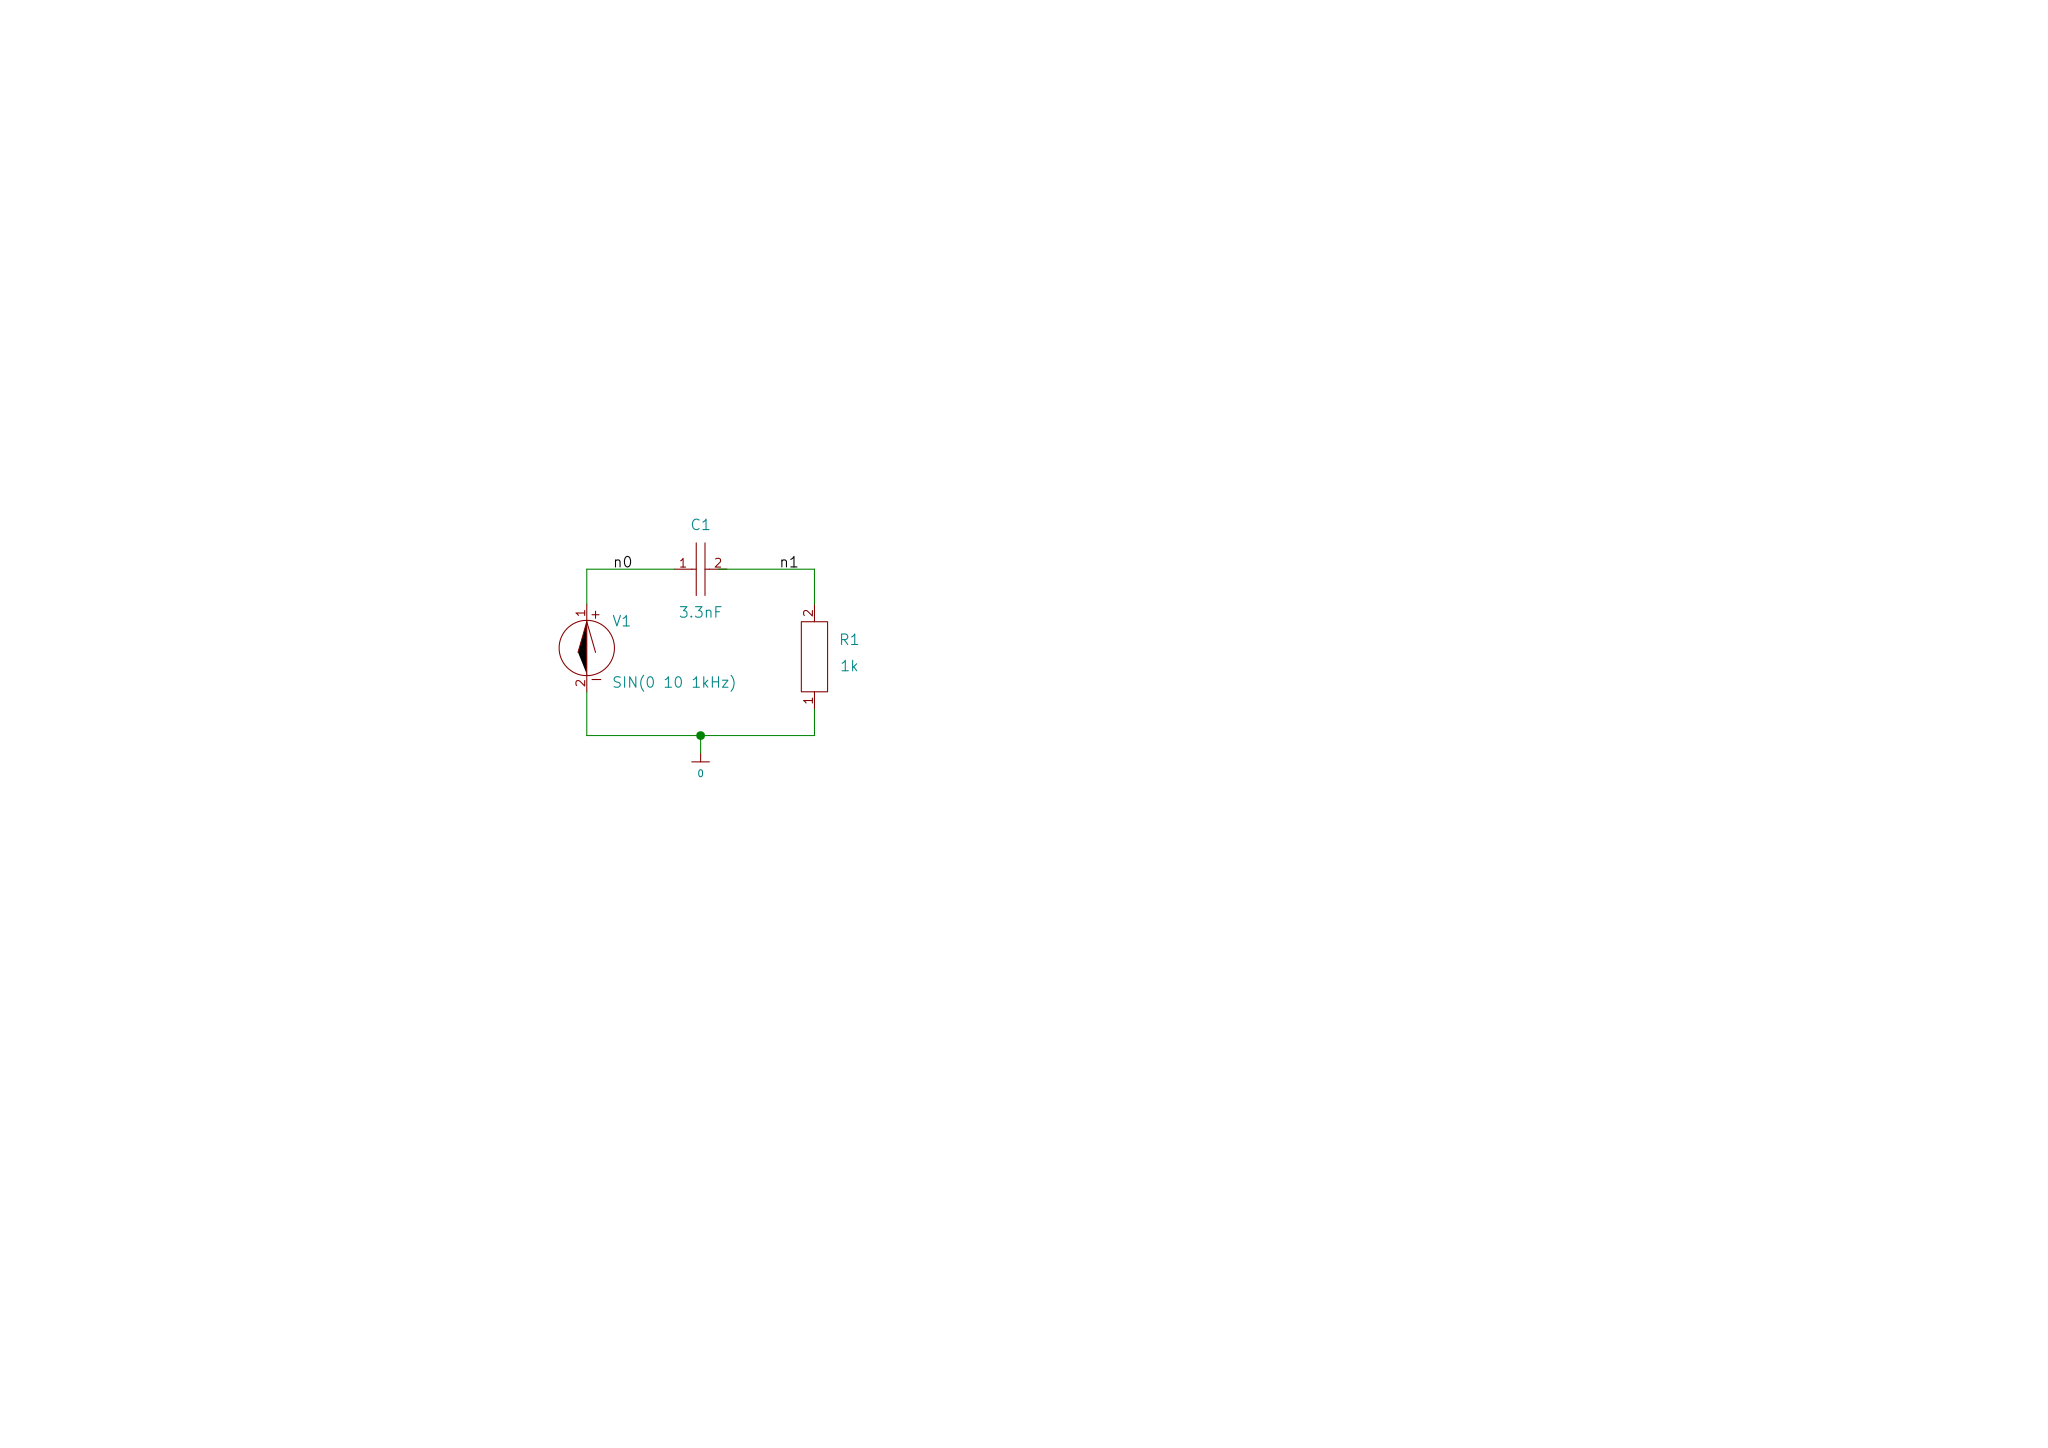
\includegraphics[height=0.5\textheight]{spice/RCfilter.pdf}
\fig{figspicerc}{Простой RC-фильтр}
\bigskip

Имена, указанные на проводниках\ --- \emph{имена цепей}. Они могут не
указываться, если вам не нужно на них ссылаться в расчете. При экспорте списка
цепей из \eeschema\ им будут присвоены униальные имена. Цепь может иметь любое
имя, за некоторым исключением: \emph{в списке должна быть одна цепь с именем
[\elem{0}], она подключается к общему проводу (земле)}. Рисуя схему, поместите
на нее один или несколько элементов [\elem{0}]\ из библиотеки \file{spice}.

\elem{V1}\ --- \term{независимый источник напряжения}. Его значение задано в
виде выражения \verb|SIN(0 10 1kHz)|, создающего синусоидальный (SIN) сигнал со
смещением (0)\,вольт, амплитудой (10)\,вольт и частотой (1kHz).

\bigskip
Рисуйте вашу схему, соблюдая несколько рекомендаций:
\begin{itemize}
  \item
Для именованных цепей используйте \emph{глобальные метки} вместо локальных.
В списке цепей глобальные идентификаторы цепей включаются как есть, а
локальные метки модифицируются, что делает сложным последующие ссылки на них при
SPICE-моделировании.
  \item
Используйте компонент [\elem{0}] из библиотеки \file{spice}, вместо обычного
комопнента [\elem{GND}]: ”\elem{0}” официальное имя главной земли в файлах
P\spice. Некоторые \spice-движки умеют транслировать $GND \rightarrow 0$, другие
нет.
\end{itemize}

\secrel{Создание списка цепей}

Входными данными для симуляции является \term{список цепей (netlist)}.
Список цепей создается через экспорт из \eeschema. Если
вы используете программу рисования схем, посмотрите в ее документации, умеет ли
она экспорт в \spice (\file{.cir}), и как это сделать.

\begin{itemize}
  \item
Кликните кнопку или пункт меню \menu{Сформирвать список цепей}.
  \item
Выберите вкладку \menu{Spice}, и убедитесь что включен крыжик \menu{\checkbox\
Формат по умолчанию}. Вам нужно сделать это только один раз, настройки
запоминаются.
\item
Нажмите кнопку \menu{Сформировать}
\end{itemize}

Если вы хотите запускать \ngs\ из диалога экспорта:
\begin{itemize}
  \item
Заполните полный путь с программе симуляции, типа
\file{C:/spice/bin/ngspice.exe} со всеми путями и расширениями, \kicad\ пока не
научился запускать симулятор через \verb|PATH|.
  \item
Нажмите кнопку \menu{Запустить симулятор}.
\end{itemize}

\bigskip
В результате экспорта будет создан файл

\lst{RCfilter.cir}{}{spice/RCfilter.cir}

Формат нетлиста \spice\ прост: каждая строка содержит один элемент схемы.
Первый столбец каждой строки содержит имя элемнта, затем идут имена цепей,
которым подключен каждый вывод, последним идет значение элемента.
Строки, наначинающиеся с [*]\ --- комментарии.
В нашем примере строка, начинающаяся с \elem{V1}, описывает источник напряжения,
подключенный к цепям \elem{n0} (вывод 1) и \elem{0} (вывод 2), значение
\verb|SIN(0 10 1kHz)|. Точно также заданы конденсатор и резистор. Так как цепи
\elem{n0,n1}\ заданы именами, перед ними стоит [/].

Первая и последняя строки имеют для \ngs\ особое значение: при чтении нетлиста
\ngs\ считает первую строку названием схемы. Последняя строка должна содержать
токен \elem{.end}.

Так как формат файла нетлиста настолько прост, его можно легко создать вручную
из любого текстового редактора. Некоторые статьи о \spice-симуляции даже
начинаются с такого способа, но он действительно неудобен для работы. Используя
\eeschema\ или другой редактор схем, намного проще изменять схему, и она может
быть легко распечетана или включена как иллюстрация в документацию. Единственный
реальный вариант, когда нужно работать напрямую в файлом\ --- если вам вдруг
понадобиться сформировать его автоматически, например при анализе паразитных
емкостей и индуктивностей печатной платы, которые определяются формой печатных
проводников.

\secrel{Запуск симуляции}

Теперь вы готовы симулировать схему. Прежде всего нам нужно решить, какие виды
расчетов, которые умеет делать \spice, нас интересуют:

\begin{itemize}
  \item \term{Анализ переходных процессов}\ показывает поведение
  схемы во времени.
  \item \term{Расчет по переменному току (AC)}\ дает измененения работы схемы с
  изменением (входой) частоты.
  \item \term{Параметрическая симуляция}\ позволяет анализировать изменения в
  работе схемы при изменении одного или нескольких параметров, например
  изменении частоты источника и емкости конденсатора.
\end{itemize}

Для начала посмотрим как ведет себя входное напряжение во времени. Мы хотим
выполнитьанализ переходных поцессов в схеме, и вывести напряжение между сетями
\elem{n0} и \elem{0}.

Запускаем \ngs:

\begin{verbatim}
$ ngspice

spinit found in c:\spice\share\ngspice\scripts\spinit
******
** ngspice-24 : Circuit level simulation program
** The U. C. Berkeley CAD Group
** Copyright 1985-1994, Regents of the University of California.
** Please get your ngspice manual from http://ngspice.sourceforge.net/docs.html
** Please file your bug-reports at http://ngspice.sourceforge.net/bugrep.html
** Creation Date: Jan 30 2012   22:58:51
******
ngspice 1 ->
\end{verbatim}

Теперь нам нужно загрузиь нетлист (выводится заголовок: первая строка файла):

\begin{verbatim}
ngspice 1 -> source RCfilter.cir

Circuit: * eeschema netlist version 1.1 (spice format) creation date: 26.12.2014 16:15:26
\end{verbatim}

Так как мы задали для входного напряжения частоту 1\,КГц, период
$T=1/F=0.001$\,с$=1$\,мс.
Мы хотим увидеть как входное наряжение меняется за первые 5 периодов, т.е.
5\,мс. Запускаем симуляцию следующей командой:

\begin{verbatim}
ngspice 2 -> tran 0.01ms 5ms
Doing analysis at TEMP = 27.000000 and TNOM = 27.000000

Warning: v1: no DC value, transient time 0 value used

Initial Transient Solution
--------------------------

Node                                   Voltage
----                                   -------
/n1                                          0
/n0                                          0
v1#branch                                    0

No. of Data Rows : 512
\end{verbatim}

Первый параметр \verb|tran| определяет \term{шаг расчета}, второй\ ---
\emph{конечное значение времени}. Если не указан третий параметр,
начальное время равно 0, иначе третий параметр указывает ненулевое
\emph{начальное время}. Ну, это все \smiley. Симуляция выполнена. Теперь нам
нужно увидеть результат симуляции.

\secrel{Просмотр результата расчета}

\spice\ создал таблицы с рассчитанными значениями: 512 значений для каждого узла
схемы. Для простого просмотра чисел выполним команду (не забудьте про кавычки,
без них не работает если первый символ [/]):

\begin{verbatim}
ngspice 3 -> plot "/n0"
\end{verbatim}

\clearpage
\noindent\includegraphics[height=\textheight]{spice/spice1.png}
\clearpage

Эта команда вывела напряжение при переходном процессе на цепи \net{n0}.

Как вы заметили, диаграмма сигнала отображается на черном фоне. Если вам нужны
другие цвета, например для вставки в документацию, их можно переопределить:

\begin{verbatim}
ngspice 12 -> set color0 = white
ngspice 13 -> set color1 = black
ngspice 14 -> set color2 = green
ngspice 3 -> plot "/n0"
\end{verbatim}

\noindent\includegraphics[height=0.5\textheight]{spice/spice2.png}

\bigskip
Диаграмма показывает форму входного сигнала, как мы и ожидали, но она нас мало
интересует, так как мы ее и задали. Нам интереснее например \emph{напряжение на
резисторе}, кроме того мы попробуем \emph{сравнить два сигнала}.
Это легко сделать указав два имени цепи:

\begin{verbatim}
ngspice 31 -> plot "/n0" "/n1"
\end{verbatim}

\clearpage
\noindent\includegraphics[height=\textheight]{spice/spice3.png}
\clearpage

\secrel{Расчет АЧХ по переменному току (AC симуляция)}

Сигнала на резисторе почти не видно. Теперь вопрос: какие частоты попускает наш
фильтр ? Для определения этого теперь выполним \term{расчет по переменному току
(AC симуляцию)}. Команда для этого\\ \verb|ac ( DEC j OCT j LIN )N FStart FEnd|.

\verb|FStart| и \verb|FEnd|\ --- соответственно начальная и конечная частота.
Необязательные параметры \verb|DEC|, \verb|OCT| или \verb|LIN| указывают способ
изменения частоты: декадно, октавно или линейно. Если выборана октавная или
декадная \term{вариация частоты}, то параметр \verb|N| задает число
частот на декаду или октаву. Для выполнения \term{AC анализа} должен быть
изменен источни сигнала: сейчас он определен как синус с амплитудой 10\,В и
частотой 1\,КГц. Для анализа это должен быть \emph{источник переменного
апряжения}. Снова запускаем \eeschema\ и меняем значение источника:

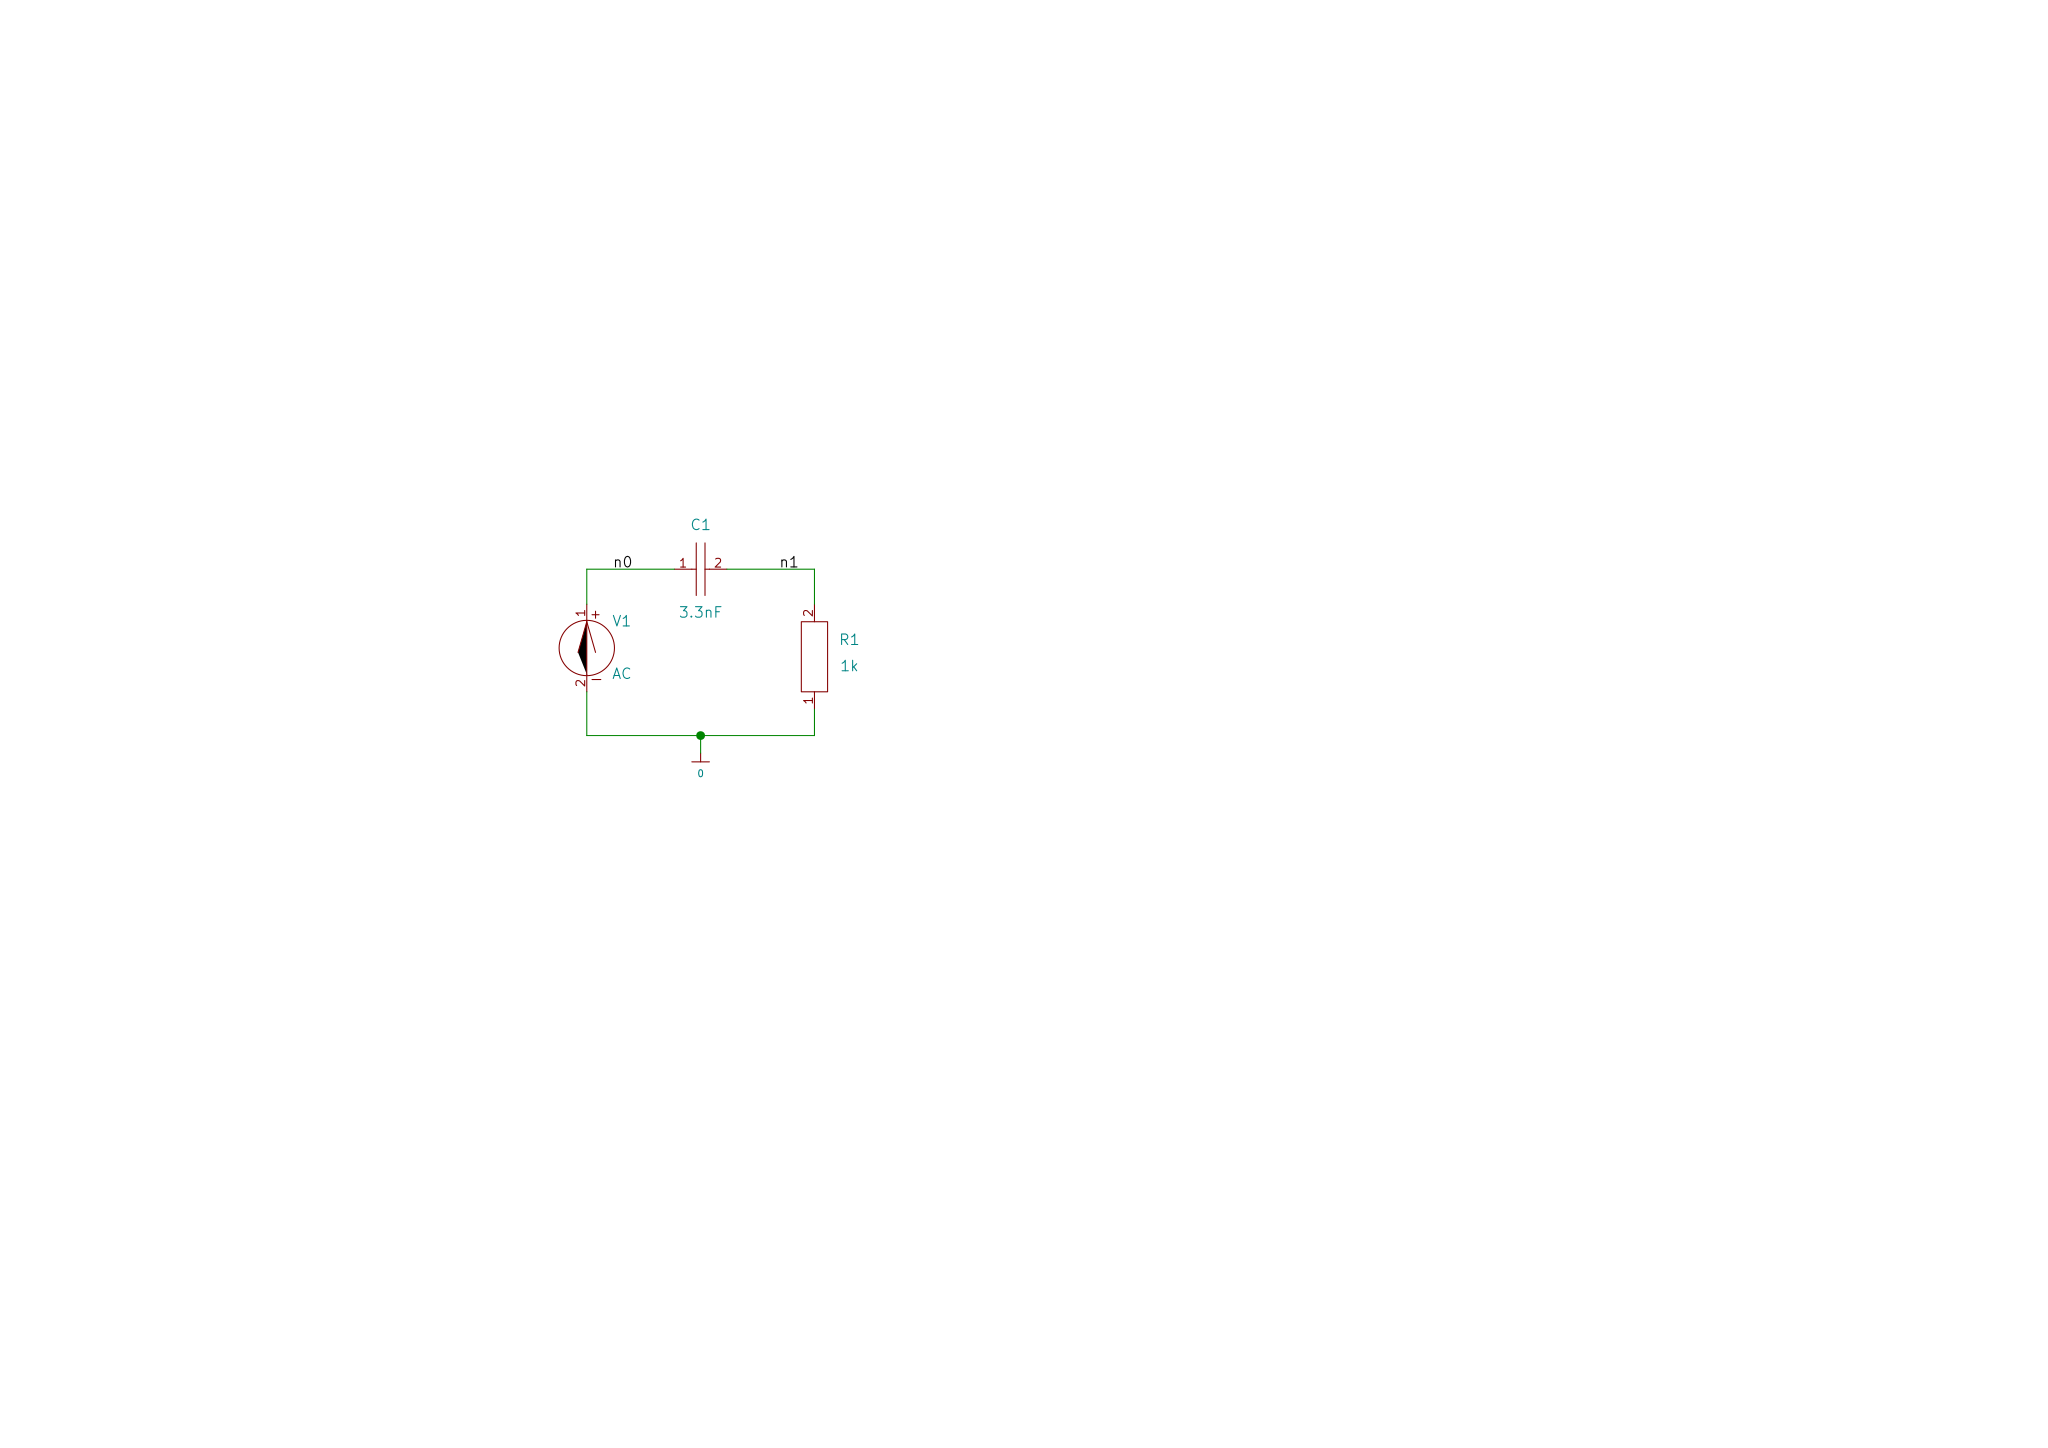
\includegraphics[height=0.5\textheight]{spice/ACanaliz.pdf}

Создаем нетлист, загружаем ео и запускаем команду AC анализа:

\begin{verbatim}
$ ngspice ACanaliz.cir
ngspice 1 -> ac lin 1000 0.1 250kHz
Doing analysis at TEMP = 27.000000 and TNOM = 27.000000

Warning: v1: has no value, DC 0 assumed


No. of Data Rows : 1000

ngspice 2 -> plot "/n1"
ngspice 3 -> plot "/n0" "/n1"
\end{verbatim}

Эта команда выполяняет \term{линейный AC анализ} от (почти) 0\,Гц до 250\,КГц.
Результат можно увидеть как напряжение для источника, так и напряжение на
\elem{R1}:

\pagebreak\noindent
\includegraphics[height=\textheight]{spice/spice4.png}

\pagebreak\noindent
\includegraphics[height=\textheight]{spice/spice5.png}

\secrel{Симуляция полноволнового выпрямителя}

\noindent
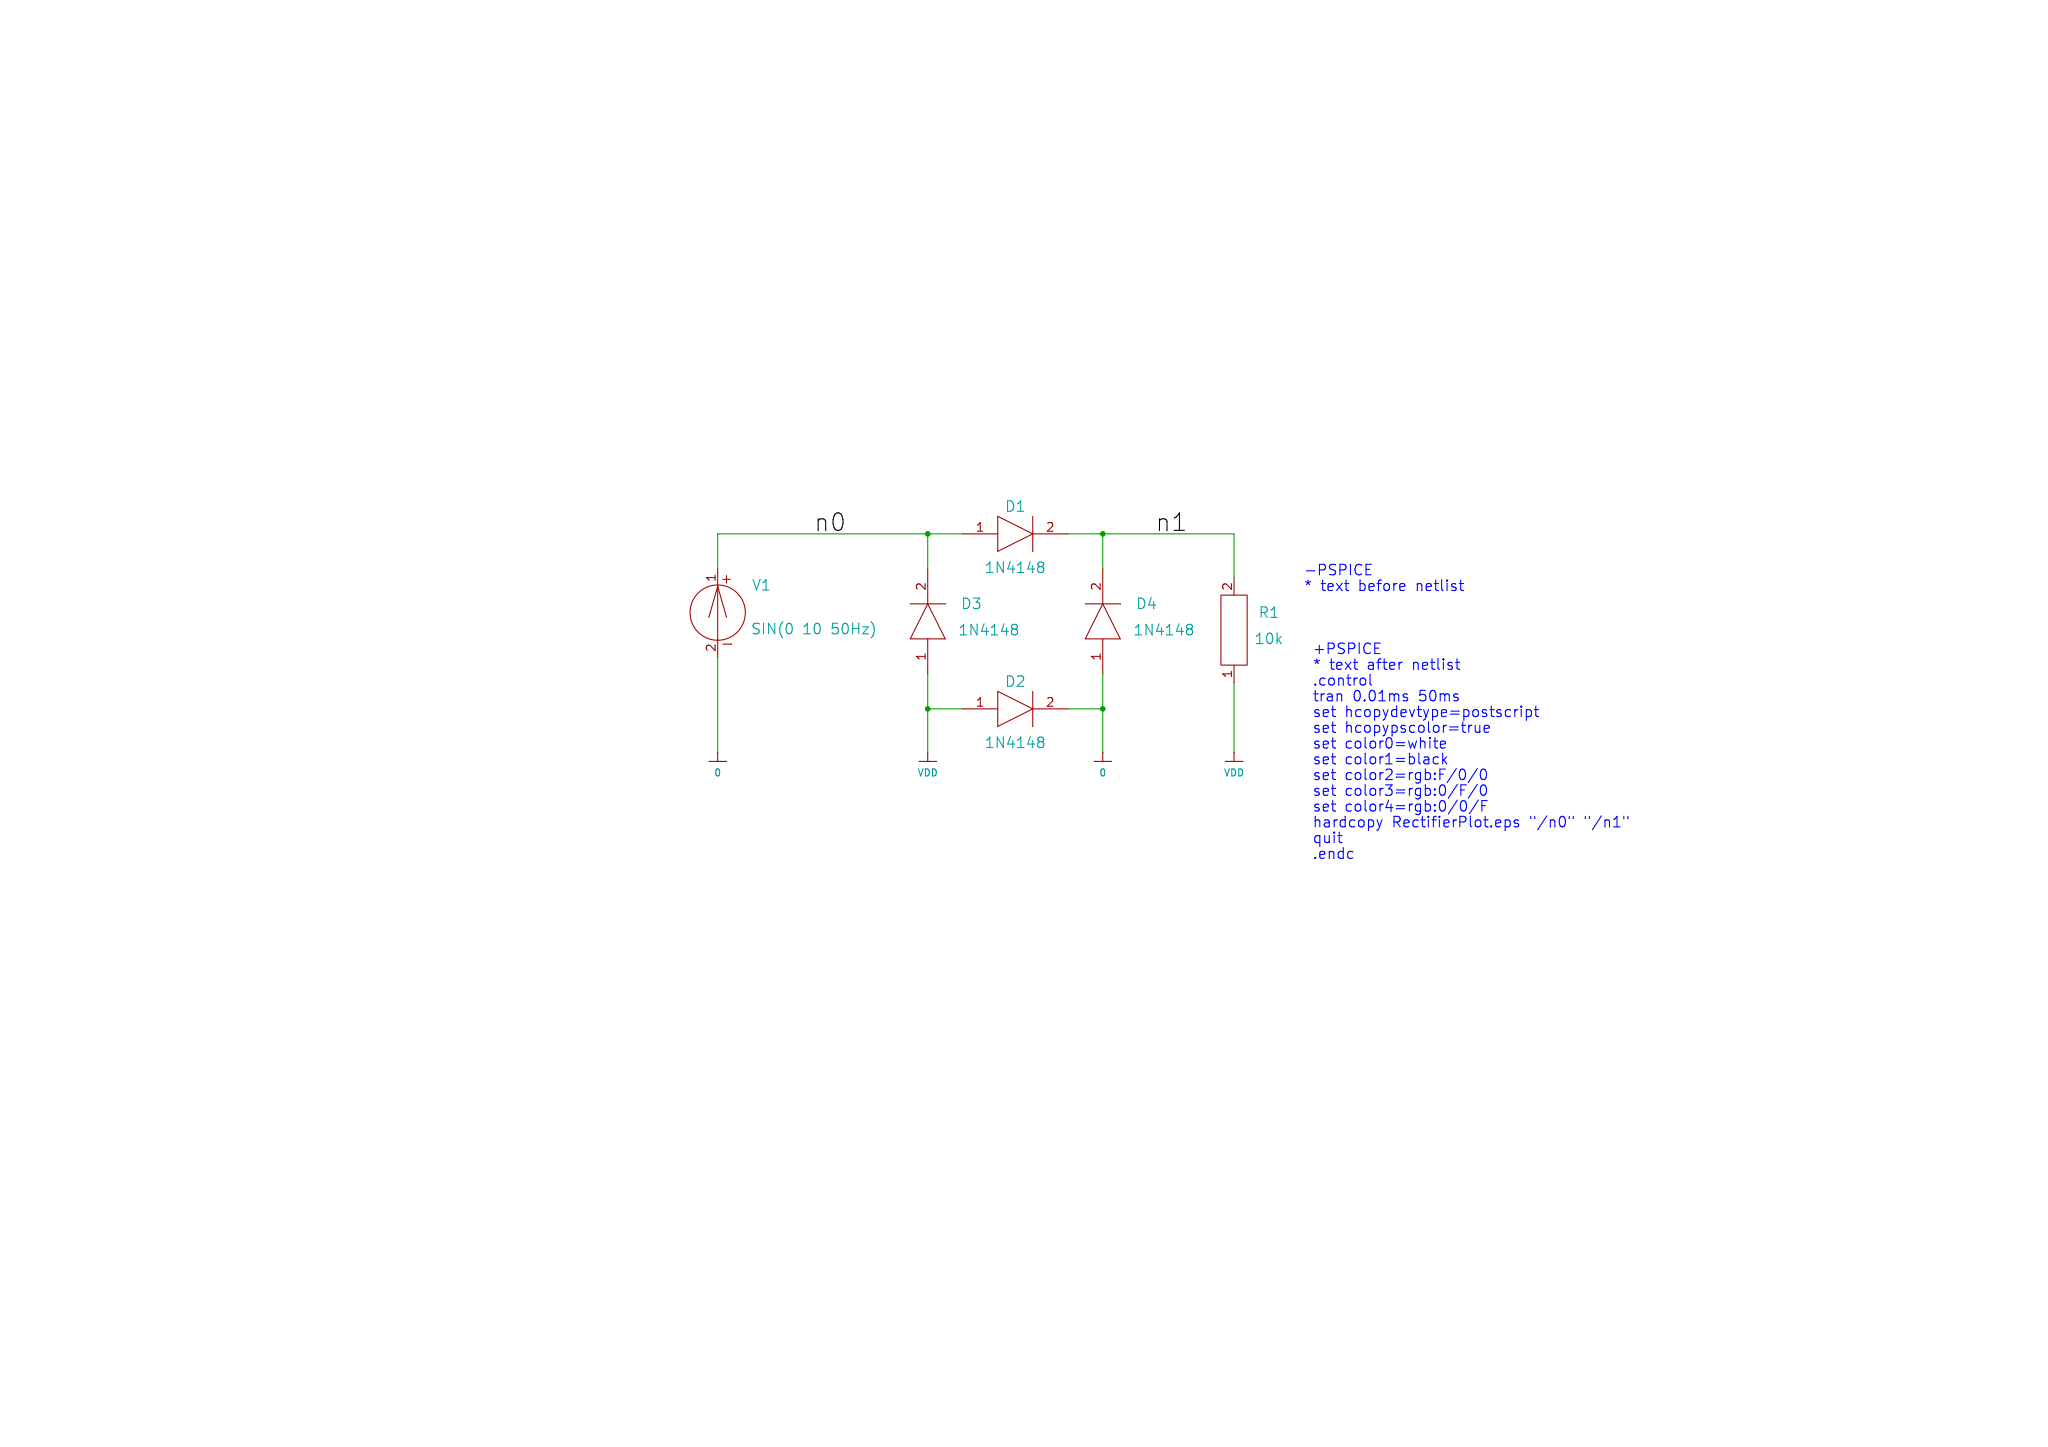
\includegraphics[width=\textwidth]{spice/Rectifier.pdf}

\lst{Rectifier.cir}{}{spice/Rectifier.cir}

Подробнее использованные здесь приемы рисования схемы описаны в \ref{kispice}.

Кратко: была применена возможность вставки в нетлист текстовых блоков до и после
списка элементов. При запуске \prog{ngspice}\ из \prog{KiCAD}\ будет
автоматически выполнен блок \verb|.control/.endc|. Также для вывода графиков
была использована команда \verb|hardcopy|, предварительно настроенная на вывод в
формате (Encapsulated) PostScript. Текущая версия \prog{ngspice} не умеет
цветной ввод, он должен быть починен в следующих версиях.

\pagebreak\noindent
\includegraphics[height=\textheight]{spice/rectifierplot.eps}

\secup


\secrel{Настройка KiCAD для SPICE-моделирования}\secdown\label{kispice}

\secrel{Библиотеки компонентов со SPICE-элементами}

\begin{itemize}
\item Библиотека базовых SPICE-компонентов поствляется с KiCAD. Эта
библиотека\ --- хороший вариант для начальных экспериментов.
Библиотека не подключена по умолчанию, вы должны сделать это вручную сами через
пенеджер библиотек. На Debian Linux это файл\\
\file{/usr/share/kicad/library/pspice.lib}\note{PSpice\ --- популярная
коммерческая версия SPICE}

\item Mithat Konar \email{webs@mithatkonar.com} разрабатывает (очень медленно)
\href{https://bitbucket.org/mithat/kicad-spice-library}{собственую
библиотеку} с некоторыми модификациями.

\item В комплекте с этой книгой поставляются библиотеки, адаптированные для
SPICE.

\end{itemize}

\secrel{Настройка проекта}

\begin{enumerate}
\item Создайте новый проект как обычно.
\item Откройте \prog{Eeschema} и удалите все библиотеки, подключаемые по
умолчанию.
\item Вручную добавьте одную из SPICE-библиотек, или набор библиотек для
этой книги. ОБратите внимание, что SPICE-библитека из поставки \prog{KiCAD}
по умолчанию не подключается к пректу.
\item Укажите расчетный SPICE-движок, который вы хотите использовать:

\menu{\prog{eeschema}>Меню>Инструменты>Сформировать список цепей>Spice}

\menu{\checkbox\ Формат по умолчанию}

\menu{\uncheckbox\ Префикс обозначений}

\menu{\checkbox\ Использовать имена цепей}

\menu{вкладка Spice>Команда симулятора:>\prog{xterm -e ngspice}}

\menu{Список цепей}

\end{enumerate}

\secrel{Как это работает}

\begin{enumerate}
  \item
Укажите режимы сиуляции, которые вы хотите выполнить, и генерацию вывода,
который хотите отобразить, добавив на схему текстовый блок (т.е.
``комментарий'') c необходимыми директивами в синтаксисе
\href{http://newton.ex.ac.uk/teaching/cdhw/Electronics2/userguide/sec5.html}{SPICE и Nutmeg}
с некоторыми добавками. Например, для выполнения \term{расчета по постоянному
току} и вывода сигнала в точке \verb|vout|, добавьте блок:
\begin{lstlisting}
+PSPICE
.control
ac dec 66 1kHz 120kHz
plot vdb(vout)
set units = degrees
plot vp(vout)
.endc
\end{lstlisting}
\begin{itemize}
  \item
Первая строка ``+PSPICE ''\ указывает kicadу добавить текст \emph{в конец}
сформированного \file{.cir}-файла. \emph{В текущей версии KiCAD есть баг,
который требует обязательного пробела после +SPICE}.
  \item
Соответственно строка ``-PSPICE ''\ добавляет текст \emph{в начало} .cir-файла.
  \item
Для поборников OpenSource, не желающих видеть ссылка на коммерческий PSpice,
предусмотрены директивы-синонимы $\pm$``GNUCAP ''. Я думаю это то же самое что и
$\pm$``PSPICE ``, но не уверен на 100\%, проверьте в документации.
  \item
Да, вам потребуется немного изучить синтакис
\href{http://newton.ex.ac.uk/teaching/cdhw/Electronics2/userguide/sec5.html}{SPICE
and Nutmeg}. Это нетрудно.
\end{itemize}
  \item
Запустите симуляцию:

\menu{\prog{eeschema}>Меню>Инструменты>Сформировать список цепей>Spice}

\menu{Запустить симулятор}

\end{enumerate}

\secup


\secup


\secrel{Разработка конструкции в САПР FreeCAD}\secdown

\includegraphics[height=0.5\textheight]{logo/FreeCAD.png}

\cp{https://ru.wikipedia.org/wiki/FreeCAD_(Juergen_Riegel\%27s)}
В среде специалистов ряда отраслей известна проблема создания полноценной САПР в
рамках OpenSource, и хотя FreeCAD ещё не является кандидатом на такую
«полноценность», этот продукт может рассматриваться как одна из попыток создания
базы для решения этой проблемы. Разработчик FreeCAD Юрген Ригель, работающий в
корпорации DaimlerChrysler, позиционирует свою программу как первый бесплатный
инструмент проектирования механики (сравнивая свой продукт с такими развитыми
проприетарными системами как CATIA версий 4 и 5, SolidWorks), созданный на
основе библиотеки \textbf{Open CASCADE}. Цель программы\ --- предоставить
базовый инструментарий этой библиотеки в интерактивном режиме.

Следует отметить, что имеет место ещё один программный продукт имеющий название
freeCAD, его разработчик\ --- Aik-Siong Koh, и он не связан с FreeCAD’ом Юргена
Ригеля.

\bigskip\cp{http://www.freecadweb.org/wiki/index.php?title=Getting\_started}
FreeCAD\ --- CAD/CAE приложение трёхмерного параметрического моделирования.
Оно в основном сделано для механического проектирования, но также может быть
использовано для любых других случаев, в которых вам нужно точно моделировать
трёхмерные объекты с контролем над историей моделирования.

FreeCAD все еще находится в ранней стадии разработки, так что, хотя он уже
предлагает Вам большой (и растущий) список функций, многого еще не хватает,
особенно если сравнивать его с коммерческими решениями, и вы можете не найти его
достаточно развитым для использования в производственной среде. Тем не менее,
есть быстрорастущее сообщество пользователей-энтузиастов, и вы уже можете найти
много примеров качественных проектов, разработанных с FreeCAD.

Как и все проекты с открытым исходным кодом, проект FreeCAD не единственый
способ работы обеспеченный Вам его разработчиками. Это во многом зависит от
роста его сообществу пользователей и разработчиком, доработки функций и
стабилизации кода (да здравствует исправление ошибок!). Так что не забывайте об
этом, когда начинаете использовать FreeCAD, если вам он нравится, вы можете
непосредственно влиять и помочь проекту!

\secrel{Установка}\secdown

\secrel{\win}

\menu{\winr>\url{http://www.freecadweb.org/}>Download>\win>\href{http://sourceforge.net/projects/free-cad/files/FreeCAD Windows/FreeCAD 0.14/}{\file{FreeCAD
0.14}}>\file{\ldots\_setup.exe}}

\menu{\file{FreeCAD 0.14.3700\_x86\_setup}>FreeCAD 0.14 License>I agree}

\menu{Distination Folder>\file{C:/FreeCAD}>Install>Completed>Close}

\menu{\winstart>Программы>FreeCAD 0.14>FreeCAD>\rms>Закрепить в панели задач}

\includegraphics[height=0.8\textheight]{freecad/about.png}

\secrel{\linux}

\secup

% \secrel{Чертеж}
% 
% \secrel{Эскиз}
% 
% \secrel{Деталь}
% 
% \secrel{Сборка}
% 
% \secrel{Автогенерация конструкторской докуметации}
% 
% \secrel{Скрипты и пользовательские расширения}
% 

\secup

\secrel{Инструменты и электронное оборудование}\secdown

\section{Радиомонтажный инструмент}

Пара надфилей, заточной камень на дрель, комплект сверел и несколько листов
наждачки.

\subsection{Pro'sKit}
Отдельного обзора заслуживает инструмент и наборы Pro'sKit
% \href{http://www.proskit.com/}{ProsKit}
%  / \href{http://www.proskit.msk.ru/index.html}{ru}.

\clearpage
\noindent\includegraphics[height=0.95\textheight]{tech/tools/proskit/PK5308BM.jpg}

\textbf{PK-5308BM универсальный набор инструментов}

\clearpage
\noindent\includegraphics[height=0.95\textheight]{tech/tools/proskit/1PK-616B.jpg}

\textbf{1PK-616B Набор инструментов для электроники профессиональный}

\clearpage\label{1PK-813B}
\noindent\includegraphics[height=0.95\textheight]{tech/tools/proskit/1PK-813B.jpg}

\textbf{1PK-813B Набор базовых инструментов для электроники}

\clearpage

По личному опыту: в 1PK-813B не хватает

\begin{itemize}
  \item мелкого мультиметра, 
  \item стриппера 1PK-3001E, 
  \item микрокусачек типа 8PK-30D, 
  \item канифоли, 
  \item ножа, 
  \item настроечную отвертку заменить индикаторной.
\end{itemize} 

\clearpage
\subsubsection{Инструмент до 1000\,В}

Для электромонтажных работ обязательно приобретите комплект
высоковольтного инструмента до 1000\,В:

\begin{tabular}{p{0.45\textwidth} p{0.45\textwidth}}
\noindent\includegraphics[width=0.45\textwidth]{tech/tools/proskit/PM-911.jpg}
&
\noindent\includegraphics[width=0.35\textwidth]{tech/tools/proskit/PM-917.jpg}
\\

\textbf{PM-911 Пассатижи 1\,кВ}
&
\textbf{PM-917 Кусачки (бокорезы) 1\,кВ}
\\
\end{tabular}
\clearpage

\subsubsection{Хранение}

\begin{tabular}{p{0.45\textwidth} p{0.45\textwidth}}
\noindent\includegraphics[width=0.45\textwidth]{tech/tools/proskit/103-132D.jpg}
&
\noindent\includegraphics[width=0.45\textwidth]{tech/tools/proskit/SB-3428SB.jpg}
\\
\textbf{103-132D Кассетница для деталей и компонентов}
&
\textbf{SB-3428SB Портативная кассетница для саморезов и т.п.}
\\
\end{tabular}
\clearpage

\subsubsection{Радиомонтаж}

\begin{tabular}{p{0.45\textwidth} p{0.45\textwidth}}
\noindent\includegraphics[width=0.45\textwidth]{tech/tools/proskit/8PK-30D.jpg}
&
\noindent\includegraphics[width=0.45\textwidth]{tech/tools/proskit/1PK-709.jpg}
\\
\textbf{8PK-30D Кусачки миниатюрные}
&
\textbf{1PK-709 Длинногубцы-кусачки}
\\
\end{tabular}
\clearpage

\begin{tabular}{p{0.45\textwidth} p{0.45\textwidth}}
\noindent\includegraphics[width=0.45\textwidth]{tech/tools/proskit/1PK-055S.jpg}
&
\noindent\includegraphics[width=0.45\textwidth]{tech/tools/proskit/1PK-29.jpg}
\\
\textbf{1PK-055S Длинногубцы изогнутые}
&
\textbf{1PK-29 Круглогубцы}
\\
\end{tabular}
\clearpage

\begin{tabular}{p{0.45\textwidth} p{0.45\textwidth}}
\noindent\includegraphics[width=0.45\textwidth]{tech/tools/proskit/1PK-101T.jpg}
&
\noindent\includegraphics[width=0.45\textwidth]{tech/tools/proskit/1PK-3001E.jpg}
\\
\textbf{1PK-101T Пинцет прямой}
&
\textbf{1PK-3001E Клещи для зачистки проводов прецизионные (стриппер)}
\\
\end{tabular}
\clearpage

\begin{tabular}{p{0.45\textwidth} p{0.45\textwidth}}
\noindent\includegraphics[width=0.45\textwidth]{tech/tools/proskit/PD-374.jpg}
&\\
\textbf{PD-374 Тиски на струбцине}
&\\
\end{tabular}
\clearpage

% \subsubsection{Прочие}
%
% Попалась интересная недорогая отвертка:
%
% \begin{multicols}{2}
% \noindent\includegraphics[width=0.90.3\textwidth]{tech/tools/proskit/P1020966.jpg}
%
% \noindent\includegraphics[width=0.90.3\textwidth]{tech/tools/proskit/P1020967.jpg}
% \end{multicols}
%
% Фиксация четкая, исполнение очень неплохое, позволяет добраться до узких мест.
% Из минусов: ручка похоже не цельнометаллическая, при изломе есть риск
% распороть руку.



\secrel{Паяльное оборудование}\secdown

\secrel{Паяльник}

Паяльник\ --- обязателен дешевый сетевой мощностью не менее 20\,Вт, типа
ЭПСН-25/220. Ограничитель мощности или регулятор температуры легко собрать
самостоятельно.

Для сборки электроники хорошо также иметь маленький монтажный 12\,В 8\,Вт от
паяльной станции ZD-927 ($\sim$100\,р), без самой станции. Если не жалко 500\,р,
берите станцию ZD-927 целиком, внутри простейший регулятор мощности, и вам не
понадобится источник питания на 12\,В, который вы еще не сделали.

\noindent\includegraphics[width=0.4\textwidth]{tech/tools/solder/EPSN25.jpg}
\textbf{Паяльник ЭПСН-25/220}

\noindent\includegraphics[width=0.4\textwidth]{tech/tools/solder/SV-55310-25.jpg}
\textbf{Паяльник 220В 25Вт, СВЕТОЗАР, SV-55310-25 230\,р.}

\noindent\includegraphics[width=0.4\textwidth]{tech/tools/solder/ZD-721N.jpg}
\textbf{Паяльник 220В 25Вт ZD-721N 175\,р.}

\noindent\includegraphics[width=0.4\textwidth]{tech/tools/solder/Iron8W.jpg}
\textbf{Паяльник для станции ZD-927 12\,В 8\,Вт 85\,р.}

\secrel{Паяльная станция}

Из всего разнообразия для хоббита оптимальным являются паяльные станции Lukey
702/853D (3000+\,р). Для работы или регулярного хобби паяльная станция с феном,
а может даже и встроенным источником питания, вещь незаменимая, и не такая уж
дорогая.

\includegraphics[width=0.45\textwidth]{tech/tools/solder/ZD927.jpg}
\textbf{Паяльная станция ZD-927 520\,р.}

\includegraphics[width=0.45\textwidth]{tech/tools/solder/Lukey702.jpg}
\textbf{Паяльная станция LUKEY 702 3100\,р.}

\clearpage
\includegraphics[width=0.95\textwidth]{tech/tools/solder/Lukey853D.jpg}

\textbf{Паяльная станция LUKEY 853D с источником питания 5200\,р.}

\secup


% \section{JTAG-адаптер}
% 
% % \input{jtag/soft}
% % \input{stlink/stlink1}
% 
% \section{Отладочные платы}
% 
% Прежде чем начать работать с отдельными \mk, устанавливая их на плату
% собственной разработки, для быстрого старта используют \term{отладочные
% платы}\note{development board, demo board}
% 
% \subsection{Arduino /Atmel Mega AVR8/}
% 
% \subsection{Cortex-Mx} %См. \ref{devkitcmx}
% 
% \subsection{CubieBoard /Cortex-A8 AllWinner A10/}
% 
% \subsection{Raspberry Pi /ARM11 BCM3032/}
% 
% \subsection{BlackSwift /MIPS/}
% 
% \subsection{VoCore /MIPS/}

\secrel{Измерительное оборудование}\secdown

\secrel{Мультиметр}\label{mmetr}

\emph{Мультиметр\ --- обязателен, без него работать невозможно}\note{или
собирать замену на паре измерительных головок тока/напряжения, и делителях}.
Для совсем начинающего больше всего подойдет M320\ref{mmetr320} c
автодиапазоном, когда освоитесь возьмете вторым прибором что-то из крупных серий
M89x/MY6x с измерением температуры\note{иногда нужно для измерения температуры
корпусов элементов, радиаторов, растворов если возитесь с электрохимией}
или ``рыльцеметр''\ref{rlcmetr} (RLC).

\secdown
\secrel{Mastech M838}\label{mmetr838}

\begin{tabular}{p{0.3\textwidth} p{0.6\textwidth}}
\noindent\includegraphics[width=0.3\textwidth]{tech/tools/mes/M838.jpg}
&
Простой, компактный, дешевый, \emph{с измерением температуры}
\\
\end{tabular}

\secrel{Mastech M300}\label{mmetr300}

\begin{tabular}{p{0.3\textwidth} p{0.6\textwidth}}
\noindent\includegraphics[width=0.3\textwidth]{tech/tools/mes/M300.jpg}
&
Простой, \emph{очень компактный}, дешевый, в чехле очень удачно умещается в
набор инструментов.
\\
\end{tabular}

\secrel{Mastech M320}\label{mmetr320}

\begin{tabular}{p{0.3\textwidth} p{0.6\textwidth}}
\noindent\includegraphics[width=0.3\textwidth]{tech/tools/mes/M320.jpg}
&
То же что и M300\ref{mmetr300}, но с \emph{автодиапазоном}, т.е. не требует
переключения диапзонов измерения вручную. На любителя, возможно \emph{удобен для
совсем начинающих}, но слишком медленен если требуется измерение меняющегося
тока/напряжения.
\\
\end{tabular}

\secup

\secrel{Осциллограф}

\secrel{Логический анализатор}

\secrel{Генератор сигналов}

\secrel{Рыльцеметр RLC}\label{rlcmetr}

\secup

\secrel{Электроинструмент}\secdown

\secrel{Дрелъ}

% \noindent
% \begin{tabular}{p{0.5\textwidth} p{0.5\textwidth}}
% \noindent
% \includegraphics[width=0.45\textwidth]{tech/tools/PraktylR.jpg}
% &
% \noindent
% \includegraphics[width=0.45\textwidth]{tech/tools/D_11_530ER.jpg}
% \\
% \textbf{Дрель ударная сетевая} & \textbf{Дрель безударная сетевая} \\
% \textbf{Praktyl-R PID13D01 400\,Вт} 
% \href{http://leroymerlin.ru/catalogue/instrumenty/elektroinstrument/dreli\_udarnye/13805983/}{\textbf{(!)395\,р.}}
% &
% \textbf{Интерскол Д-11/530ЭР (с БЗП)}
% \href{http://leroymerlin.ru/catalogue/instrumenty/elektroinstrument/dreli\_bezudarnye/11857763/}{\textbf{1120\,р.}}
% \\
% \end{tabular}
% \bigskip
% 
% Дрель\ --- одноразовая китайчатина от 400\,р. Продаются уже брендированные на
% Леруа Мерлен, наклейка <<PID13D01 Ударная дрель 400\,Вт, 13\,мм>>. Скорость
% регулируется глубиной нажатия курка, крутилка на курке ограничивает глубину
% механически, фиксатор держит скорость близко к минимальной, запаха горелой
% пластмассы через несколько минут работы на холостом ходу нет.
% 
% По надежности рекомедуется Интерскол 1100+\,р. Надежность Интерскола\ --- не
% <<китай>>, классика ДУ-580ЭР работает в хвост и гриву, используется криворукими
% студентами, лежит в подвале в пыли от точила, и никаких вопросов даже со
% щетками.
% 
% Если не планируете много сверлить бетон, \textbf{берите дрель без ударного
% механизма}: отсутствуют лишние продольные перемещения, что может быть важно при
% использовании в качестве шпинделя сверлильного станка, и механизации других
% технологических поделок.
% 
% У шуруповерта нет 43\,мм шейки для фиксации, поэтому как средство электропривода
% он практически бесполезен, и нужен собственно для заворачивания большого
% количества саморезов. Хотя наличие ограничителя крутящего момента и малые
% габариты удобны при сверлении и сборке поделок.
% 
% \bigskip
% Имея некоторое количество поделочного материала, кривые руки и особенно доступ к
% станочному оборудованию, можно сколкозить некоторое подобие настольных
% станочков\ \pref{fig:drelstans}\ для механизации некоторых работ,
% используя дрель в качестве привода.
% 
% Главным элементом такой оснастки\ --- зажим на шейку дрели 43\,мм. Особых
% требований по его точности и качеству нет, т.к. сама шейка обычно пластиковая, и
% никакой доводки по круглости и параллельности оси инструмента не проходит.
% 
% \clearpage
% \phantomsection\label{fig:drelstans}
% \noindent\includegraphics[height=0.528\textheight]{tech/tools/DrelLathe.jpg}
% \noindent\includegraphics[height=0.528\textheight]{tech/tools/DrelShliph.jpg}
% 
% \noindent\includegraphics[height=0.465\textheight]{tech/tools/DrelLathe2.jpg}
% \noindent\includegraphics[height=0.465\textheight]{tech/tools/DrelBoren.jpg}
% \clearpage

\secrel{Лобзик}

% \noindent
% \begin{tabular}{p{0.5\textwidth} p{0.5\textwidth}}
% \noindent
% \includegraphics[width=0.45\textwidth]{tech/tools/LobzPraktyl.jpg}
% &
% \noindent
% \includegraphics[width=0.45\textwidth]{tech/tools/LobzMakita4329.jpg}
% \\
% \href{http://leroymerlin.ru/catalogue/instrumenty/elektroinstrument/lobziki/13805991/}{\textbf{Praktyl
% 350 Вт 356\,р.}} 
% & 
% \href{http://leroymerlin.ru/catalogue/instrumenty/elektroinstrument/lobziki/12114283/}{\textbf{Makita
% 4329 2260\,р.}}
% \\
% \end{tabular}
% \bigskip
% 
% Лобзик полезен при разделке стеклотекстолита, и изготовлении технологической
% мебели (стеллажи, рабочие столы и т.п.).

\secrel{Жвигатель}

% Если у вас возникло желание механизировать изготовление механических деталей, а
% свободного доступа к настоящему станочному оборудованию нет, есть смысл
% рассмотреть изготовление самодельной механизированной оснастки 
% типа\ \pref{fig:drelstans}, или даже самодельных станочков. В этом случае надо
% рассмотреть применения универсального привода.
% 
% Первый кандидат на место универсального электропривода достается той самой
% дрели, не забываем об обязательном наличии 43\,мм монтажной шейки.
% Достоинство дрели как привода\ --- прямое подключение к сети, встроенный
% редуктор, есть модели с простой регулировкой оборотов, есть резьба и отверстие
% под винт на валу, в комплекте есть патрон для зажима мелких деталей в
% точилке\footnote{\ БЗП удобен, патрон с ключем дает лучший зажим и возможно
% точнее}.
% 
% Ограниченно доставаемые двигатели от стиральных машин, отличаются мощностю и
% оборотистостью, особенно от старых моделей. Часто доступны сразу с готовым
% шкивом на валу, который иногда проще использовать, чем снять.
% 
% Автозапчасти: привод печки Камаза, двигатель постоянного тока 
% 24\,В 50\,Вт
% 
% Новые асинхронные двигатели АИРЕ 56 B2/B4 (3000/1500 об.) с заводским
% конденсатором, подключается к сети $\sim$220\,В, цена от 2500\,р.
% С ростом размеров и мощности цена резко повышается.
% Следует обратить внимание на возможность монтажа на дополнительный фланцевый
% подшипниковый щит, (?) с моделями АИРЕ 80.
% 
% Для самодельных серлилок и микроинструмента хороши китайские воздушные шпиндели
% постоянного тока с цанговыми патронами ER11. Требуют источник питания
% постоянного тока 9$\div$48\,В. В магазинах не попадались, необходима прямая
% покупка с \href{http://www.aliexpress.com/}{AliExpress}\note{пользуйтесь
% английской версией\ --- переводная жуткое УГ}\ по почте.
% 
% % \clearpage
% \begin{tabular}{l l}
% 
% \noindent\includegraphics[width=0.37\textwidth]{tech/tools/VyatkaDvig.jpg} 
% & 
% \noindent\includegraphics[width=0.37\textwidth]{tech/tools/KamazDvig.jpg}
% \\
% \textbf{Жвигатель Вятка-Автомат 19??\,г.}
% &
% \textbf{Двигатель печки Камаза}
% \\
% 
% \noindent\includegraphics[width=0.37\textwidth]{tech/tools/AIRE.jpg}
% & 
% \noindent\includegraphics[width=0.37\textwidth]{tech/tools/ER11.jpg}
% \\
% \textbf{АИРЕ 56 B2, 0.2\,КВт}
% &
% \textbf{Воздушный шпиндель с цангой ER11}
% \\
% 
% \end{tabular}
% \clearpage
% 
% Съемные фрезерные шпиндели, поставляются отдельно или в комплекте с насадкой
% ручного фрезера по дереву. Лучшие, со стальной шейкой\ --- Kress, активно
% применяются хобби-ЧПУшниками. Попроще и сильно дешевле делал Интерскол, иногда
% попадается noname. Недостаток как универсального привода\ --- они
% высокоскоростные, возникают проблемы с понижающими передачами. Применение\ ---
% приводной высокоскоростной инструмент: боры, фрезы по дереву, микроинструмент
% для граверов (микродиски, шарошки). Цанга 8\,мм. Для некоторых моделей бывают
% наборы цанг на мелкий инструмент.
% 
% \bigskip
% \begin{tabular}{p{0.3\textwidth} p{0.3\textwidth} p{0.3\textwidth} }
% \noindent\includegraphics[height=0.3\textheight,width=0.3\textwidth,keepaspectratio]{tech/tools/Kress530.jpg}
% &
% \noindent\includegraphics[height=0.3\textheight,width=0.3\textwidth,keepaspectratio]{tech/tools/Interskol30.jpg}
% &
% \noindent\includegraphics[height=0.3\textheight,width=0.3\textwidth,keepaspectratio]{tech/tools/InterskolFM55.jpg}
% \\
% KRESS 530/800/1050 FM(E)
% &
% Интерскол ФМ-30/750
% &
% Интерскол ФМ-55/1000 Э
% \\
% \href{http://kress-shop.ru/product/frezernyj-dvigatel-530-fm-kress-06082302/}{5600+\,р.}
% &
% /снят с производства/
% &
% \href{http://www.kuvalda.ru/catalog/1867/27920/}{5050\,р.}
% \\
% \end{tabular}

\secup



\secup


\secrel{Станочное оборудование}\label{stanki}
\secdown

\input{tabletop/tabletop}

\secrel{Самодельная оснастка и станки}
\secdown

\secrel{Сверлилка из китайского шпинделя}

\secrel{Ручной резьбонарезной стенд}

\secrel{Намоточный станок}

\secup


\secrel{Промышленные станки}\secdown

% Самый распространенные станки\ --- \term{сверлильные}, т.к. имеют самую простую
% конструкцию, и минимальную стоимость. Предназначены для самой частой операции:
% изготовления перпендикулярных круглых дырок в различных материалах, топовые
% модели имеют также функцию нарезения резьбы.
% 
% \bigskip
% 
% Наиболее многочисленную группу металлорежущих станков составляют \term{токарные
% станки}, используются в механических, инструментальных и ремонтных цехах
% заводов, а также в ремонтных мастерских в основном для обработки деталей,
% имеющих форму тел вращения. При использовании соответствующей оснастки позволяют
% растачивать отверстия в призматических (прямоугольных) деталях, и фрезеровать
% небольшие детали. Самый ходовой тип детали\ --- тело вращения с наружними и
% внутренними резьбами: валики, втулки, оси, болты, винты, шпильки, кольца, шайбы
% и т.д.
% 
% К основным размерам, характеризующим токарный станок, относятся 
% \begin{itemize}
%   \item наибольший допустимый диаметр обрабатываемой заготовки, 
%   \item высота \term{центров} над станиной и 
%   \item расстояние между центрами.
%   \item 
% Часто обращают внимание на диаметр \emph{проходного отверстия шпинделя},
% определяющий максимальный диаметр \term{длинномерных заготовок}, что важно при
% изготовлении мелких партий деталей или нарезке резьб на трубах.
% \end{itemize}
% 
% \bigskip
% Значительную часть среди металлорежущих станков составляют \term{фрезерные
% станки}. Наибольшее распространение имеют консольно-фрезерные.
% Предназначены для выполнения различных фрезерных работ цилиндрическими,
% дисковыми, фасонными и другими \term{фрезами}, можно фрезеровать плоскости,
% пазы, фасонные поверхности, и т.д. Кроме этого, универсальные
% консольно-фрезерные станки c поворотным столом или делительной головкой
% позволяют фрезеровать различного рода винтовые канавки и зубья зубчатых колес.
% 
% Основными размерами фрезерных станков, по которым можно определить возможность
% установки и обработки конкретных заготовок с определенными габаритами, являются
% размеры рабочей поверхности стола (длина и ширина) и \emph{рабочий ход
% стола}/\term{рабочая зона} в продольном, поперечном и вертикальном направлениях.

\secrel{Маркировка моделей станков производства СССР}

% \begin{tabular}{p{0.3\textwidth} p{0.6\textwidth}}
% \includegraphics[height=0.3\textheight]{stanki/chugunok.jpg}
% &
% станок-''чугунок'', простой, дубовый, надежный (потому что ненадежные давно
% сломались), дешевый, но требует помещение с силовым полом, 3х-фазное питание, и
% кучу времени на поиск запчастей для восстановления по металлобазам и развалам. В
% диком виде пока что встречается в школах и других типа учебных заведениях, т.к.
% висит на балансе, но не эксплуатируется, и не обслуживается, потому что некем.
% Отличается дешевизной (ржавого) инструмента и (еще более ржавой) оснастки, и
% некоторым гемором с поиском запчастей.
% \\
% \end{tabular}
% \clearpage
% 
% 
% Для станков, выпускавшихся в СССР, принята единая система классификации и
% условных обозначений, основанная на присвоении каждому станку особого шифра
% (номера). Cтанки каждой группы подразделяются на девять \emph{типов}.
% Внутри каждого типа металлорежущие станки могут отличаться друг от друга
% конструктивными особенностями. Эти особенности, а также некоторые другие
% характеристики и отражаются в шифре (номере) станка.
% 
% \begin{verbatim}
% <группа>[<буква1>]<тип><характеризующий размер>[<буква2>][M][Фn]
% \end{verbatim}
% 
% Кроме цифр, в условные обозначения модели станка часто входят буквы. Если
% \emph{буква1} стоит между первой и второй цифрами, то это означает, что
% конструкция станка подверглась усовершенствованию по сравнению с прежней
% моделью. 
% 
% Если \emph{буква2} стоит в конце номера станка, то это говорит об
% изменении основной, «базовой» модели станка. Часто \emph{буква2} задает класс
% точности:
% 
% \begin{description}
% \item[Н] нормальная (часто не указывается)
% \item[П] повышенная
% \item[В] высокая
% \item[А] особо высокая
% \item[С] особо-точный станок
% \end{description}
% 
% Для станков с ЧПУ:
% \begin{description}
% \item[М] наличие магазина инструментов,
% \item[Ф1] станки с цифровой индикацией и преднабором координат,
% \item[Ф2] с позиционными и прямоугольными системами,
% \item[Ф3] с контурными системами,
% \item[Ф4] с универсальной системой для позиционной и контурной обработки. Эти
% шифры пишутся в конце номера модели.
% \end{description}
% 
% \bigskip
% \noindent\emph{группа}/\emph{тип}:
% \begin{enumerate}[label={\arabic*}]
%   \item токарные;
%   \begin{enumerate}[label={\arabic*}]
%     \item 
%     \item 
%     \item револьверные;
%     \item 
%     \item 
%     \item токарно-винторезные;
%   \end{enumerate}
%   \item сверлильные и расточные;
%   \begin{enumerate}[label={\arabic*}]
%     \item вертикально-сверлильные,
%     \item одношпиндельные полуавтоматы,
%     \item многошпиндельные полуавтоматы,
%     \item координатно-расточные,
%     \item радиально-сверлильные,
%     \item горизонтально-расточные,
%     \item алмазно-расточные,
%     \item горизонтально-сверлильные,
%     \item разные сверлильные.  
%   \end{enumerate}
%   \item шлифовальные, полировальные, доводочные и заточные;
%   \item специальные;
%   \item зубо- и резьбообрабатывающие;
%   \item фрезерные;
%   \item разрезные;
%   \item строгальные, долбежные, протяжные;
%   \item прочие
% \end{enumerate}
% 
% \bigskip
% \term{Характеризующий размер}:
% \begin{description}
% \item[токарные] \hfill \\
% высота оси шпинделя над станиной, \\
% задает \emph{максимально возможный радиус} обрабатываемой \emph{заготовки}
% \end{description}
% 
% \bigskip
% Пример: 1А616: станок токарно(1)-винторезный(6), модификация(А), высота
% центров над станиной (16)0 мм.

\clearpage
\secrel{\odina: станок токарно-винторезный}\label{latheodina}\secdown

\includegraphics[height=0.5\textheight]{stanki/1A616.jpg}

\secrel{Назначение и области применения}

\secrel{Распаковка и транспортировка}

\secrel{Фундамент станка, монтаж и установка}

\secrel{Подготовка станка к первоначальному пуску}

\secrel{Паспортные данные}

\secrel{Описание основных узлов}

\secrel{Смазка}

\secrel{Первоначальный пуск}

\secrel{Указания по технике безопасности}

\secrel{Настройка}

\secrel{Регулирование}

\secrel{Ведомость комплектации}

\secup


\secup

\secup


\secrel{Разработка ПО для встраиваемых систем}\secdown

% \chapter{Архитектура программных систем}

\section{Ортогональность}

\cp{http://ru.wikibooks.org/wiki/\%D0\%9E\%D1\%80\%D1\%82\%D0\%BE\%D0\%B3\%D0\%BE\%D0\%BD\%D0\%B0\%D0\%BB\%D1\%8C\%D0\%BD\%D0\%BE\%D1\%81\%D1\%82\%D1\%8C}

\term{Ортогональность}\ очень важна, если вы хотите создавать системы, которые
легко поддаются проектированию, сборке, тестированию и расширению. Однако этому
принципу редко обучают непосредственно. Часто он является лишь скрытым
достоинством других разнообразных методик, которые вы изучаете. Это неправильно.
Как только вы научитесь непосредственно применять принципы ортогональности, вы
сразу заметите, как улучшилось качество создаваемых вами систем.

\paragraph{Что такое ортогональность?}

Термин "ортогональность"\ заимствован из геометрии. Две линии являются
ортогональными, если они пересекаются под прямым углом, например, оси координат
на графике. В терминах векторной алгебры две \emph{такие линии перемещения
являются независимыми}. Если двигаться параллельно оси X вдоль одной из линий,
то проекция движущейся точки на другую линию не меняется. Этот термин был введен
в информатике для обозначения некой разновидности независимости или
несвязанности. В грамотно спроектированной системе программа базы данных будет
ортогональной к интерфейсу пользователя: вы можете менять интерфейс пользователя
без воздействия на базу данных и менять местами базы данных, не меняя
интерфейса. Перед тем как рассмотреть преимущества ортогональных систем,
познакомимся с неортогональной системой.

\paragraph{Неортогональная система}

Предположим, вы находитесь в экскурсионном вертолете, совершающем полет над
Гранд-Каньоном, когда пилот, который совершил ошибку, наевшись рыбы за обедом
внезапно вскрикивает и теряет сознание. По счастливой случайности это
происходит, когда вы парите на высоте 30 метров. Вы догадываетесь, что рычаг
управления общим шагом несущего винта обеспечивает подъем машины, так что, если
его слегка опустить, вертолет начнет плавно снижаться. Однако когда вы пытаетесь
сделать это, то осознаете, что жизнь\ --- не такая уж простая штука. Вертолет
клюет носом, и вас начинает вращать по спирали влево. Внезапно вы понимаете, что
управляете системой, в которой каждое воздействие имеет побочные эффекты. При
нажатии на левый рычаг вам придется сделать уравновешивающее движение назад
правым рычагом и нажать на правую педаль. Но при этом каждое из этих действий
вновь повлияет на все органы управления. Неожиданно вам приходится жонглировать
невероятно сложной системой, в которой любое изменение влияет на все остальные
управляющие воздействия. Вы испытываете феноменальную нагрузку: ваши руки и ноги
находятся в постоянном движении, пытаясь уравновесить все взаимодействующие
силы. Органы управления вертолетом определенно не являются ортогональными.

\paragraph{Преимущества ортогональности}

Как показывает пример с вертолетом, неортогональные системы сложнее изменять и
контролировать. Если составляющие системы отличаются высокой степенью
взаимозависимости, то невозможно устранить какую-либо неисправность лишь на
локальном уровне.

\bigskip
\emph{Исключайте взаимодействие между объектами, не относящимися друг к другу}
\bigskip

Мы хотим спроектировать компоненты, которые являются самодостаточным
независимыми, с единственным, четким назначением. Когда компоненты изолированы
друг от друга, вы уверены, что можно изменить один из них, не заботясь об
остальных. Пока внешние интерфейсы этого компонента остаются неизменными можете
быть спокойны, что не создадите проблем, которые распространятся по
\emph{всей}\ системе. С созданием ортогональных систем у вас появятся два
больших преимущества: увеличение производительности и снижение риска.

\paragraph{Увеличение производительности}

\begin{itemize}
\item Изменения в системе локализуются, поэтому периоды разработки и
тестирования сократятся. Легче написать относительно небольшие, самодостаточные
компоненты, чем один большой программный модуль. Простые компоненты могут быть
спроектированы, запрограммированы, протестированы и затем забыты\ --- не нужно
непрерывно менять существующий текст по мере того, как к нему добавляются новые
фрагменты.

\item Ортогональный подход также способствует многократному использованию
компонентов. Если компоненты имеют определенную, четкую сферу ответственности,
они могут комбинироваться с новыми компонентами способами, которые не
предполагались при их первоначальной реализации. Чем меньше связанность в
системах, тем легче их перенастроить и провести их обратное проектирование.

\item При комбинировании ортогональных компонентов происходит заметное
увеличение производительности. Предположим, что один компонент способен
осуществлять М, а второй\ --- N различных операций. Если эти компоненты
ортогональны и комбинируются, то в сумме они способны осуществить $M\times N$
различных операций. Но если два компонента не являются ортогональными, они будут
перекрываться, и результат их действия будет меньшим по сравнении с
ортогональными компонентами. Вы получаете большее количество функциональных
возможностей в пересчете на единичное усилие, если комбинирует между собой
ортогональные компоненты.
\end{itemize}

\paragraph{Снижение риска}

Ортогональный подход приводит к снижению уровня риска, присущего любой
разработке.

\begin{itemize}
\item Ошибочные фрагменты текста программы изолируются. Если модуль содержит
ошибку, то вероятность ее распространения на всю систему уменьшается. Кроме
того, ошибочный фрагмент может быть извлечен и заменен новым (исправленным).

\item Конечный продукт (система) становится менее хрупким. Проблемы,
появляющиеся при внесении небольших изменений и устранении недочетов на
определенном участке, не проходят дальше этого участка.

\item Ортогональная система способствует повышению качества тестирования,
поскольку облегчается проектирование и тестирование отдельных ее компонентов.

\item Вы не будете слишком сильно привязаны к определенному субподрядчику,
программному продукту или платформе, поскольку интерфейсы между компонентами,
производимыми фирмами-субподрядчиками, не будут играть главенствующей роли в
проекте.
\end{itemize}




\secrel{VCS: cистемы контроля версий}\label{vcs}\secdown

\secrel{CVS}

\secrel{Subversion}

\secrel{Git}
\secdown

\secrel{GitHub}

\secup

\secup


\chapter{Вспомогательные скрипты на языке \py}

\begin{tabular}{p{0.1\textwidth} p{0.8\textwidth}}
\includegraphics[width=0.1\textwidth]{python/logo.png}&
\emph{
Название языка произошло вовсе не от вида пресмыкающихся. Автор назвал язык в
честь популярного британского комедийного телешоу 1970-х «Летающий цирк Монти
Пайтона». Впрочем, всё равно название языка чаще ассоциируют именно со змеёй,
нежели с передачей\ --- пиктограммы файлов в KDE или в Microsoft Windows и даже
эмблема на сайте \url{http://www.python.org} (до выхода версии 2.5) изображают
змеиные головы.
}
\\
\end{tabular}
\bigskip

\py\note{в оригинале читается \textbf{п\'{а}йтон}, но давно русифицировался как
\textbf{пит\'{о}н}}\ --- высокоуровневый язык программирования общего
назначения, ориентированный на повышение производительности разработчика и
читаемости кода.

\py\ удобно применять для написания различных вспомогательных скриптов.
Часто его используют при разработке сложных программных систем для написания
первых версий. В процессе работы над большими программами часто перерабатываются
большие объемы кода, поэтому для ускорения разработки требуется максимально
высокоуровневый язык. После того как архитектура программы стабилизируется,
узким местом становится производительность, и программу переписывают на более
низкоуровневом компилируемом языке, чаще всего \cpp.

Написание программ упрощают:

\begin{itemize}
  \item \textbf{объектно-ориентированное программирование} облегчает разработку
  программ, позволяет переопределить стандартные операторы для пользовательских
  типов данных, упрощая синтаксис
  \item \textbf{динамическая типизация} не требуется заранее упределять
  переменные, они создаются простым присваиванием
  \item \textbf{обработка исключений} для секции кода можно определить
  обработчик ошибок
  \item \textbf{высокоуровневые структуры данных}\ --- списки, словари (набор
  элементов ключ:значение), очереди
  \item богатая стандартная библиотека и множество дополнительных библиотек на
  все случаи
\end{itemize}

\section{Установка под \win}\label{pywinstall}

\bigskip
\menu{
\keys{\winstart+R}
>
\url{http://www.python.org}
>
Downloads
>
\href{https://www.python.org/ftp/python/2.7.8/python-2.7.8.msi}{Python 2.7.8}
}

\bigskip
\menu{\file{python-2.7.8.msi}
>
Setup>
for all users/for me
}

\menu{Destination Directory > \file{C:/Python/} > Next}

\nopagebreak
\bigskip
\includegraphics[width=0.45\textwidth]{python/install/037.png}
\includegraphics[width=0.45\textwidth]{python/install/038.png}
\bigskip


\menu{Customize > Python > Add python.exe to PATH > Next > Finish}

\nopagebreak
\bigskip
\includegraphics[width=0.45\textwidth]{python/install/039.png}
\includegraphics[width=0.45\textwidth]{python/install/045.png}
\bigskip

\section{Дополнительные материалы}

\cite{pyotkidach} Г. Россум, Ф.Л.Дж. Дрейк, Д.С. Откидач, 
\href{http://rus-linux.net/MyLDP/BOOKS/python.pdf}{Язык программирования Python}

\cite{pythink} Аллен Дауни
\href{https://drive.google.com/file/d/0B0u4WeMjO894Q2hWV1QwOFFQOVk/view?usp=sharing}{Думать
на языке \py: Думать как компьютерный специалист}



% \chapter{Make: управление сборкой проектов}\label{make}
% 
\secrel{Основы Си и \cpp}\secdown
\secup


% \subsection{Установка MinGW (win32)}
% 
% \section{Особенности \cpp\ в embedded}
% 
% \chapter{LLVM и разработка собственных компиляторов}
% 
% \secrel{Лексический и синтаксический анализ}\secdown

Очень часто в практике возникает необходимость работы с данными в текстовых
форматах\ --- \termdef{plain text}{plain text} файлы, в которых в каком-либо
формате (на языке разметки, или \termdef{DDL}{DDL}: \termdef{[D]ata
[D]efinition [L]anguage}{Data Definition Language}) описаны данные. И от вас
требуется реализовать разбор такого файла, выделяя синтаксические структуры и
элементы данных, чтобы в дальнейшем после их преобразования например записать
текстовый файл в другом формате.

В таком виде хранятся результаты расчетных программ, работащих в пакетном
режиме, данные с измерительных систем, поток данных с приемников
GPS\note{протокол NMEA 0183}, очень популярный мета-формат XML со всеми его
частными случаями типа HTML, XLIFF\ref{xliff}, OpenDocument, тексты программ
для станков с ЧПУ,\ldots

С некоторыми хинтами точно так же можно работать и с бинарными файлами,
преобразовав их сначала в текстовую форму (в простейшем случае просто сделав hex
dump).

В некоторых случаях необходимо написание трансляторов форматов (текстовых)
данных, или даже интерпретаторов/компиляторов языков программирования.

\bigskip
Все эти техники с использованием стандартных утилит \prog{flex}\ и \prog{bison}\
будут кратко описаны в этой главе. Подробнее эти техники рассмотрены в
книгах\ref{lexlit}, особенно стоит отметить талмуд
\textbf{DragonBook}:

\bigskip

\label{exdragon}\cite{dragonbook} \textbf{Книга Дракона}: Ахо, Сети, Ульман
Принципы построения компиляторов.

\bigskip

\href{http://habrahabr.ru/post/99162/}{Habr: Компиляция. 1: лексер}

\href{http://habrahabr.ru/post/99298/}{Habr: Компиляция. 2: грамматики}

\href{http://habrahabr.ru/post/99366/}{Habr: Компиляция. 3: бизон}

\href{http://habrahabr.ru/post/99397/}{Habr: Компиляция. 4: игрушечный ЯП}

\href{http://habrahabr.ru/post/99466/}{Habr: Компиляция. 5: нисходящий разбор}

\href{http://habrahabr.ru/post/102597/}{Habr: Компиляция. $5\frac{1}{2}$: llvm
как back-end}

\href{http://habrahabr.ru/post/99592/}{Habr: Компиляция. 6: промежуточный код}


\secrel{Лексер и лексический анализ, утилита \prog{flex}}

\begin{framed}
\noindent
\termdef{Л\'{е}ксер}{лексер}/\termdef{сканер}{сканер}\ --- программа или ее
часть, которая \begin{enumerate}[nosep]
  \item
получает на вход исходные
данные в виде сплошного потока одиночных сиволов,
  \item
группирует символы согласно
набору правил (заданных \termdef{регулярными выражениями}{регулярное
выражение}) и
  \item
отдает на выходе символы, уже сгруппированные в \termdef{лекс\'{е}мы}{лексема}\
или \termdef{ток\'{е}ны}{токен}.
\end{enumerate}
Цель лексера\ --- подготовить последовательность лексем для входа другой
программы. \\
В самый простых случаях на лексер можно возложить простые преобразования текста.
\end{framed}

\termdef{Лексический анализ}{лексический анализ}\ --- процесс программного
разбора входной последовательности символов\note{например, такой как исходный
код на одном из языков программирования} с целью получения на выходе
последовательности групп символов\ --- \term{токенов}, имеющих собственное
смысловое значение\note{подобно группировке букв в слово}. Как правило,
лексический анализ производится в соответствии набора правил определённого
\term{формального, искуственного или компьютерного языка}.

\begin{framed}\noindent
\term{Компьютерный язык}, а точнее его \termdef{грамматика}{грамматика}, задаёт
определённый набор лексем, которые могут встретиться на входе лексера, и набор
правил, по которым их следует группировать.
\end{framed}

Традиционно принято организовывать процесс лексического анализа, рассматривая
входную последовательность символов как поток одиночных символов. При такой
организации \term{лексер}\ самостоятельно управляет выборкой отдельных символов
из входного потока.

Распознавание лексем с учетом грамматики обычно производится путём их
идентификации согласно идентификаторам токенов, определяемых грамматикой языка.
При этом любая последовательность символов входного потока (лекс\'{е}ма),
которая согласно грамматике не может быть идентифицирована как токен языка,
обычно рассматривается как специальный \term{токен-ошибка}.

\bigskip
Каждый выделенный токен можно представить в виде парной структуры,
содержащей
\begin{enumerate}
  \item идентификатор токена и
  \item саму последовательность символов лексемы, выделенной из входного
потока\note{запись строки, числа и т. д.}.
\end{enumerate}

\bigskip
Рассморим обработку текстового файла: разделение текстового фрагмента на абзацы,
запись в формате
\href{http://docs.oasis-open.org/xliff/xliff-core/xliff-core.html}{XLIFF} для
перевода в системе \href{http://smartcat.pro}{ABBYY SmartCAT}, и обратной
трансляции из XLIFF в \LaTeX-совместимое форматирование.

\bigskip
Так как задача построения \termdef{лексических анализаторов}{лексический
анализатор} является стандартной задачей информатики, был разработан типовой
инструмент: \term{генератор лексических анализаторов} \prog{flex}. Эта программа
транслирует описание лексера на своем высококоуровневом языке в фрагмент
программы на языке Си/\cpp\ или самостоятельную программу. Описание лексера
прописывается в \file{.lex}-файле в формате:

\begin{verbatim}
определения, опции, декларации
%%
правила выделения токенов через регулярки
%%
сишный код
\end{verbatim}

\paragraph{Комментарии} поддерживаются сишные \verb|/* */| комментарии.

\paragraph{Опции} \verb|%option|

\bigskip\noindent
\begin{tabular}{l l}
noyywrap & отключает вызов лексером функции \verb|yywrap()| при достижении
конца текущего файла \\
main & включение типовой функции \verb|main()| вместо заданной пользователем \\
case-insensitive & регистро-независимый лексический анализ, большие/маленькие
буквы не различаются \\
yylineno & в глобальной си-переменной \verb|yylineno| доступен номер
текущей строки \\
\end{tabular}

\paragraph{Формат опреления} \verb|имя определение|:
\begin{verbatim}
digit    [0-9]
number   [\+\-]{0,1}{digit}+\.{digit}*
\end{verbatim}

\paragraph{Декларации на Си} прописываются в скобках \verb|%{ }%|

\cp{http://matt.might.net/articles/standalone-lexers-with-lex/}

\lst{xliff/txt/txt2xliff.lex}{}{xliff/txt/txt2xliff.lex}

\secrel{Генератор синтаксических анализаторов \prog{bison}}

\begin{framed}
\termdef{Синтаксический анализ}{синтаксический анализ}\ --- процесс анализа
последовательности токенов с определением их грамматической структуры. На этом
этапе выделяются \term{синтаксичекие ошибки}.
\end{framed}

\secrel{Семантический анализ}

\begin{framed}
\termdef{Семантический анализ}{семантический анализ}\ --- процесс выполнения
\term{семантических проверок}: контроль типов, привязка объектов и т.д. 
\end{framed}

\secrel{Оптимизация}

Выполнение формальных преобразований структур данных, описываютщих
компилируюемую программу, с целью построения более компактного/быстрого
машинного кода.

\secrel{Кодогенерация}

Получение реального машинного кода в бинарном представлении, или в виде
ассемблерных текстовых файлов.

\secrel{Дополнительная литература}\label{lexlit}

\bigskip

\url{http://alumni.cs.ucr.edu/~lgao/teaching/flex.html}

\url{http://www.capsl.udel.edu/courses/cpeg421/2012/slides/Tutorial-Flex\_Bison.pdf}

\secrel{Транслятор Паскаля}

\secrel{LLVM и разработка собственных компиляторов}

\secup

% 
% \chapter{Сборка кросс-компилятора GNU toolchain}

\secup


\secrel{Микроконтроллеры \cmx}
\secdown

\secrel{Производители}\secdown
\secrel{ST Microelectronix STM32}\secdown
\secup

\input{cortex/lpc}
\input{cortex/milandr}
\secup


\secrel{Отладочные платы}\secdown

\secrel{LeafLabs Maple Mini: STM32F103 /\cm{3}/}
\secdown
\secup


\input{muino/muino}

\secrel{Серия STM32 STM32DISCOVERY}\secdown
\secrel{STM32DISCOVERY: STM32F103 /\cm{3}/}

\secrel{STM32F4DISCOVERY: STM32F406 /\cm{4F}/}

\secrel{STM32F0DISCOVERY: STM32F040 /\cm{0}/}

\secup

\secup

% \label{devkitcmx}
% 
% \secdown
% 
% \secrel{STM32DISCOVERY /\cm{3} STM32F103/}
% 
% \secrel{STM32F4DISCOVERY /\cm{4} STM32F407/}
% 
% \secrel{Maple Mini /\cm{3} STM32F100/}
% 
% \secup

\secup


\secrel{Встраиваемый em\linux}\secdown

% Linux для встраиваемых систем\note{будем называть его \emlinux}\ ---
популярный метод быстрого создания комплекса ПО для больших сложных приложений,
работающих на достаточно мощном железе, особенно предполагающих интенсивное
использование сетевых технологий.

За счет использования уже существующей и очень большой базы исходных текстов
ядра, библиотек и программ для \linux, бесплатно доступных в т.ч. и для
коммерческих приложений, можно на порядки сократить стоимость разработки
собственных программных компонентов, и при этом получить готовую команду
бесплатных стронних разработчиков, уже знакомых с созданием ПО для \linux.

Из недостатков можно отметить:
\begin{itemize}
  \item Отсутствие полноценной поддержки режима жесткого реального времени;
  \item Тяжелое ядро;
  \begin{itemize}
  \item Поддерживаются только мощные семейства процессоров\note{32-бит,
  необходим блок MMU};
  \item Значительные требования по объему \ram\ и общей производительности;
  \end{itemize}
  \item Дремучесть техспециалистов, контуженных ТурбоПаскалем и
Win\-dows\-ом;
\end{itemize}

Для \term{сборки}\ \emlinux-системы используется метод \term{кросс-компиляции},
когда используется \term{кросс-тулчейн}, компилирующий весь комплект ПО для
компьютера с другой архитектурой. Типичный пример\ --- сборка ПО на
ПК c процессором Intel i7 для Raspberry Pi или планшета на процессоре
AllWinner/Tegra/\ldots.

\emlinux\ очень широко применяется на рынке мобильных устройств\note{в т.ч.
является основой Android}, и устройств интенсивно использующих сетевые протоколы
(роутеры, медиацентры).

В качествe примера применения рассмотрим относительно простое приложение:
многофункциональные настенные часы с синхронизацией времени через \internet, с
будильником, медиапроигрывателем, блэкджеком и плюшками.

% UI vesamenu.c32
MENU RESOLUTION 640 480
MENU TITLE azLinux
MENU BACKGROUND /syslinux/splash640x480.png

DEFAULT memtest
LABEL memtest
MENU LABEL memtest86+
KERNEL /syslinux/memtest.krn

LABEL debian
MENU LABEL Debian GNU/Linux amd64 netinst
KERNEL /Debian/vmlinuz
INITRD /Debian/initrd.gz
APPEND vga=none



\chapter{azLinux}

Чтобы разобраться

\section{Поддерживаемое железо}

\begin{tabular}{|l| l l|l l l l l|}
\hline
HW & CPU & ARCH & RAM & HDD/NAND & SD & USB & WiFi \\
\hline
qemu386 & i486sx & i386 & 32M+ & \uncheckbox\ IDE/SATA & & \uncheckbox &\\
eeepc701 & CeleronM & i386 & 512M+ & \uncheckbox\ SSD 4G & \uncheckbox\
SD & \checkbox & \uncheckbox\ Atheros AR2425 \\
\hline
qemuARM & & arm & 32M+ &&&&\\
cubie1 & AllWinnerA10 & armhf & 1G && \uncheckbox\ $\mu$SD & \checkbox &\\
rpi & BCM2835 & armel & 512M && \uncheckbox\ SD&\checkbox&\\
\hline
mr3020 & AR7240 &mips& 32M & 4M & & \checkbox & \uncheckbox\ Atheros AR9331 \\
\hline
\end{tabular}

% \section{Конфигурации процессоров}


% \chapter{Библиотека libSDL}\secdown

Библиотека \href{http://www.libsdl.org/}{SDL} предоставляет такие средства, как
быстрый вывод 2D-графики, обработку ввода, проигрывание звука, вывод 3D через
OpenGL и другие операции, причем делает это кросплатформенно. Список платформ
обширный: Linux, Windows, Windows CE, BeOS, Mac OS X, FreeBSD, NetBSD, OpenBSD,
BSD/OS, Solaris, IRIX и QNX\ --- и вдобавок есть неофициальные порты на другие
системы.

Сама библиотека написана на Си и поддерживает \cpp, однако есть биндинги к
большинству популярных языков. Автор \prog{libsdl} был нанят компанией Valve,
программные продукты которой активно используют библиотеку. К тому же, теперь
библиотека выходит под лицензией zlib, а не LGPLv2, как было раньше, и SDL 2.0
можно использовать в любых своих приложениях, в т.ч. коммерческих Скорее всего
сделано это было для того, чтобы Valve смогла включить ее в Steam для Linux.

\bigskip
Использование SDL позволяет писать графические и мультимедийные приложения для
em\linux, не включая в систему достаточно тяжелую X Window System.

\bigskip
В книге рассмотрена версия 1.2.15, последняя версия из ветки \prog{SDL1}, т.к.
она используется в сборке az\linux\ \ref{azlin}. Сейчаc активно развивается
ветка \prog{SDL2}, ее особенности кратко рассмотрены в разделе \ref{sdl2}.

\secrel{Инициализация и завершение SDL-программы}

\begin{verbatim}
int main() {
	...
	SDL_Init(SDL_INIT_xxx));
	...
	SDL_Quit();
}
\end{verbatim}

\begin{description}
\item[SDL\_INIT\_EVERYTHING] все подсистемы, не работает с отключенным звуком
\item[SDL\_INIT\_VIDEO] только графическая подсистема
\end{description}

\secrel{LazyFoo tutorial}\secdown

\cp{http://lazyfoo.net/SDL\_tutorials/}

\secrel{Setting up SDL and Getting an Image on the Screen}

Since SDL is a third party library, you have to install it yourself. Here you'll
get a step by step guide on how to set it up.

If you have any problems try consulting the
\href{http://www.libsdl.org/faq.php}{SDL Development FAQ}.

Once you set up SDL, you can move on the second half of the tutorial and learn
to load and show images on the screen.

\secdown
\secrel{\win}

An important note for Visual Studio users: The latest version of SDL for visual
studio comes with two sets of library and binary files: x86 for 32bit, x64 for
64bit. If you're on a 64bit operating system, Visual Studio still compiles in
32bit by default. When you set the library directory, it should point to the x86
folder inside of the lib folder.

\bigskip
Установка для следующих сред разработки описана
\href{http://lazyfoo.net/SDL_tutorials/lesson01/windows/index.php}{здесь}:

\begin{enumerate}
  \item Dev C++ 4.9.9.2
  \item Code::Blocks 8.02
  \item MinGW Developer Studio 2.05
  \item Eclipse 3.1
  \item Command Line (MinGW)
  \item Visual Studio.NET 2010 Express
  \item Visual Studio.NET 2005/2008 Express
  \item Visual Studio.NET 2003
\end{enumerate}

\secrel{\linux}

Пакеты ставятся из вашего дистрибутива. 

Для включения в az\linux\ добавьте пакет \pack{sdl}\ в переменную
конфигурирования \verb|LIBS += sdl|. Сборка пакета описана в \ref{azsdl}.

\secrel{Getting an Image on the Screen}

This tutorial covers how to do Hello World SDL style.

Now that you have SDL set up, it's time to make a bare bones graphics
application that loads and displays an image on the screen.

\begin{verbatim}
// Include SDL functions and datatypes
#include "SDL/SDL.h"
\end{verbatim}

At the top of the source file we include the SDL header file so we can use the
SDL functions and data types.

Remember that some of you (like Visual Studio users) are going to include SDL
like this:

\begin{verbatim}
#include "SDL.h"
\end{verbatim}

So if the compiler is complaining that it can't find "SDL/SDL.h", then it's
either because you're including the wrong path or you forgot to put SDL.h in the
right place.

\begin{verbatim}
int main( int argc, char* args[] )
{
    //The images
    SDL_Surface* hello = NULL;
    SDL_Surface* screen = NULL;
\end{verbatim}

At the top of the main() function, two SDL\_Surface pointers are declared. An
SDL\_Surface is an image, and in this application we're going to be dealing with
two images. The surface "hello" is the image we're going to be loading and
showing. The "screen" is what is visible on the screen.

Whenever you're dealing with pointers, you should always remember to initialize
them.

Also, when using SDL, you must have your main() function declared like it is
above. You can't use void main() or anything like that.

\begin{verbatim}
    //Start SDL
    SDL_Init( SDL_INIT_EVERYTHING );

    //Set up screen
    screen = SDL_SetVideoMode( 640, 480, 32, SDL_SWSURFACE );

    //Load image
    hello = SDL_LoadBMP( "hello.bmp" );
\end{verbatim}

The first function we call in the main() function is SDL\_Init(). This call of
SDL\_Init() initializes all the SDL subsystems so we can start using SDL's
graphics functions.

Next SDL\_SetVideoMode() is called to set up a 640 pixel wide, 480 pixel high
window that has 32 bits per pixel. The last argument (SDL\_SWSURFACE) sets up
the surface in software memory. After SDL\_SetVideoMode() executes, it returns a
pointer to the window surface so we can use it.

After the window is set up, we load our image using SDL\_LoadBMP().
SDL\_LoadBMP() takes in a path to a bitmap file as an argument and returns a
pointer to the loaded SDL\_Surface. This function returns NULL if there was an
error in loading the image.

\begin{verbatim}
    //Apply image to screen
    SDL_BlitSurface( hello, NULL, screen, NULL );

    //Update Screen
    SDL_Flip( screen );

    //Pause
    SDL_Delay( 2000 );
\end{verbatim}

Now that we have our window set up and our image loaded, we want to apply the
loaded image onto the screen. We do this using SDL\_BlitSurface(). The first of
SDL\_BlitSurface() argument is the source surface. The third argument is the
destination surface. SDL\_BlitSurface() sticks the source surface onto the
destination surface. In this case, it's going to apply our loaded image onto the
screen. You'll find out what the other arguments do in later tutorials.

Now that our image is applied to screen, we need to update the screen so we can
see it. We do this using SDL\_Flip(). If you don't call SDL\_Flip(), you'll only
see an unupdated blank screen.

Now that the image is applied to the screen and it's made visible, we have to
make the window stay visible so it doesn't just flash for a split second and
disappear. We'll make the window stay by calling SDL\_Delay(). Here we delay the
window for 2000 milliseconds (2 seconds). You'll learn a better way to make the
window stay in place in tutorial 4.

\begin{verbatim}
    //Free the loaded image
    SDL_FreeSurface( hello );

    //Quit SDL
    SDL_Quit();

    return 0;
}
\end{verbatim}

Now that we're not going to use the loaded image anymore in our program, we need
to remove it from memory. You can't just use delete, you have to use
SDL\_FreeSurface() to remove the image from memory. At the end of our program,
we call SDL\_Quit() to shut down SDL.

You may be wondering why we never deleted the screen surface. Don't worry,
SDL\_Quit() cleans it up for you.

Congratulations, you've just made your first graphics application.

\secrel{Troubleshooting your SDL application}

If the compiler complains that it can't find 'SDL/SDL.h', it means you forgot to
set up your header files. Your compiler/IDE should be looking for the SDL header
files, so make sure that it's configured to look in the SDL include folder.

If you're using Visual Studio and the compiler complains 'SDL/SDL.h': No such
file or directory, go to the top of the source code and make sure it says
\verb|#include "SDL.h"|.

If your program compiles, but linker complains it can't find some lib files,
make sure your compiler/IDE is looking in the SDL lib folder. If your linker
complains about an undefined references to a bunch of SDL functions, make sure
you linked against SDL in the linker.

If your linker complains about entry points, make sure that you have the main
function declared the right way and that you only have one main function
combined in your source code.

If the program compiles, links, and builds, but when you try to run it it
complains that it can't find SDL.dll, make sure you put SDL.dll in the same
directory as the compiled executable. Visual Studio users will need to put the
dll file in the same directory as your vcproj file. Windows users can also put
the dll inside of the system32 directory.

If you run the program and the images don't show up or the window flashes for a
second and you find in stderr.txt:

\begin{verbatim}
Fatal signal: Segmentation Fault (SDL Parachute Deployed)
\end{verbatim}

It's because the program tried to access memory it wasn't supposed to. Odds are
its because it tried to access NULL when SDL\_BlitSurface() was called. This
means you need to make sure the bitmap files are in the same directory as the
program. Visual Studio users will need to put the bitmap file in the same
directory as your vcproj file.

Also if you're using Visual Studio and you get the error "The application failed
to start because the application configuration is incorrect. Reinstalling the
application may fix this problem.", it's because you don't have the service pack
update installed. Do not forget to have the latest version of your compiler/IDE
with the service pack update for your compiler/IDE or SDL will not work with
Visual Studio.

Some Linux users will run and get a blank screen. Try running the program from
the command line.

If you had to create a project to compile an SDL program, remember that you will
need to create a project for every SDL program you create. Or, better yet, you
can reuse the SDL project you made the first time.
Download the media and source code for this tutorial here.

\secup

\secrel{Optimized Surface Loading and Blitting}

Now that you got an image on the screen in part 2 of the last tutorial, it's
time do your surface loading and blitting in a more efficient way.

\begin{verbatim}
//The headers
#include "SDL/SDL.h"
#include <string>
\end{verbatim}

Here are our headers for this program.

SDL.h is included because obviously we're going to need SDL's functions.

The string header is used because ... eh I just like 
\verb|std::string over char*|

\begin{verbatim}
//The attributes of the screen
const int SCREEN_WIDTH = 640;
const int SCREEN_HEIGHT = 480;
const int SCREEN_BPP = 32;
\end{verbatim}

Here we have the various attributes of the screen.

I'm pretty sure you can figure out what SCREEN\_WIDTH and SCREEN\_HEIGHT are.
SCREEN\_BPP is the bits per-pixel. In all of the tutorials, 32-bit color will be
used.

\begin{verbatim}
//The surfaces that will be used
SDL_Surface *message = NULL;
SDL_Surface *background = NULL;
SDL_Surface *screen = NULL;
\end{verbatim}

These are the three images that are going to be used.

"background"\ is obviously going to be the background image, "message"\ is the
bitmap that says "Hello"\ and "screen"\ is obviously the screen.

Remember: its a good idea to always set your pointers to NULL if they're not
pointing to anything.

\begin{verbatim}
SDL_Surface *load_image( std::string filename )
{
    //Temporary storage for the image that's loaded
    SDL_Surface* loadedImage = NULL;

    //The optimized image that will be used
    SDL_Surface* optimizedImage = NULL;
\end{verbatim}

Here we have our image loading function.

What this function does is load the image, then returns a pointer to the
optimized version of the loaded image.

The argument "filename"\ is the path of the image to be loaded. "loadedImage"\
is the surface we get when the image is loaded. "optimizedImage"\ is the surface
that is going to be used.

\begin{verbatim}
    //Load the image
    loadedImage = SDL_LoadBMP( filename.c_str() );
\end{verbatim}

First the image is loaded using SDL\_LoadBMP().

But it shouldn't be used immediately because the bitmap is 24-bit. The screen is
32-bit and it's not a good idea to blit a surface onto another surface that is a
different format because SDL will have to change the format on the fly which
causes slow down.

\begin{verbatim}
    //If nothing went wrong in loading the image
    if( loadedImage != NULL )
    {
        //Create an optimized image
        optimizedImage = SDL_DisplayFormat( loadedImage );

        //Free the old image
        SDL_FreeSurface( loadedImage );
    }
\end{verbatim}

Next we check if the image was loaded properly. If there was an error,
loadedImage will be NULL.

If the image loaded fine, SDL\_DisplayFormat() is called which creates a new
version of "loadedImage"\ in the same format as the screen. The reason we do
this is because when you try to stick one surface onto another one of a different
format, SDL converts the surface so they're the same format.

Creating the converted surface every time you blit wastes processing power which
costs you speed. Because we convert the surface when we load it, when you want
to apply the surface to the screen, the surface is already the same format as
the screen. Now SDL won't have to convert it on the fly.

So now we have 2 surfaces, the old loaded image and the new optimized image.

SDL\_DisplayFormat() created a new optimized surface but didn't get rid of the
old one.

So we call SDL\_FreeSurface() to get rid of the old loaded image.

\begin{verbatim}
    //Return the optimized image
    return optimizedImage;
}
\end{verbatim}

Then the newly made optimized version of the loaded image is returned.

\begin{verbatim}
void apply_surface( int x, int y, SDL_Surface* source, SDL_Surface* destination )
{
    //Make a temporary rectangle to hold the offsets
    SDL_Rect offset;

    //Give the offsets to the rectangle
    offset.x = x;
    offset.y = y;
\end{verbatim}

Here we have our surface blitting function.

It takes in the coordinates of where you want to blit the surface, the surface
you're going to blit and the surface you're going to blit it to.

First we take the offsets and put them inside an SDL\_Rect. We do this because
SDL\_BlitSurface() only accepts the offsets inside of an SDL\_Rect.

An SDL\_Rect is a data type that represents a rectangle. It has four members
representing the X and Y offsets, the width and the height of a rectangle. Here
we're only concerned about x and y data members.

\begin{verbatim}
    //Blit the surface
    SDL_BlitSurface( source, NULL, destination, &offset );
}
\end{verbatim}

Now we actually blit the surface using SDL\_BlitSurface().

The first argument is the surface we're using.

Don't worry about the second argument, we'll just set it to NULL for now.

The third argument is the surface we're going to blit on to.

The fourth argument holds the offsets to where on the destination the source is
going to be applied.

\begin{verbatim}
int main( int argc, char* args[] )
{
\end{verbatim}

Now we start the main function.

When using SDL, you should always use:

\begin{verbatim}
int main( int argc, char* args[] )
\end{verbatim}

or

\begin{verbatim}
int main( int argc, char** args )
\end{verbatim}

Using int main(), void main(), or any other kind won't work.

\begin{verbatim}
    //Initialize all SDL subsystems
    if( SDL_Init( SDL_INIT_EVERYTHING ) == -1 )
    {
        return 1;
    }
\end{verbatim}

Here we start up SDL using SDL\_Init().

We give SDL\_Init() SDL\_INIT\_EVERYTHING, which starts up every SDL subsystem.
SDL subsystems are things like the video, audio, timers, etc that are the
individual engine components used to make a game.

We're not going to use every subsystem but it's not going to hurt us if they're
initialized anyway.

If SDL can't initialize, it returns -1. In this case we handle the error by
returning 1, which will end the program.

\begin{verbatim}
    //Set up the screen
    screen = SDL_SetVideoMode( SCREEN_WIDTH, SCREEN_HEIGHT, SCREEN_BPP, SDL_SWSURFACE );
\end{verbatim}

Now it's time to make our window and get a pointer to the window's surface so
we can blit images to the screen.

You already know what the first 3 arguments do. The fourth argument creates the
screen surface in system memory.

\begin{verbatim}
    //If there was an error in setting up the screen
    if( screen == NULL )
    {
        return 1;
    }
\end{verbatim}

If there was a problem in making the screen pop up, screen will be set to NULL.

\begin{verbatim}
    //Set the window caption
    SDL_WM_SetCaption( "Hello World", NULL );
\end{verbatim}

Here the caption is set to "Hello World".

The caption is this part of the window:

\begin{verbatim}
    //Load the images
    message = load_image( "hello.bmp" );
    background = load_image( "background.bmp" );
\end{verbatim}

Now the images are loaded using the image loading function we made.

\begin{verbatim}
    //Apply the background to the screen
    apply_surface( 0, 0, background, screen );
\end{verbatim}

Now it's time to apply the background with the function we made.

Before we blitted the background, the screen looked like this:

But now that we blitted the background image, the screen looks like this in
memory:

When you blit, you copy the pixels from one surface onto another. So now the
screen has our background image in the top left corner, but we want to fill up
the entire screen. Does that mean we have to load the background image 3 more
times?

\begin{verbatim}
    apply_surface( 320, 0, background, screen );
    apply_surface( 0, 240, background, screen );
    apply_surface( 320, 240, background, screen );
\end{verbatim}

Nope. We can just blit the same surface 3 more times.

\begin{verbatim}
    //Apply the message to the screen
    apply_surface( 180, 140, message, screen );
\end{verbatim}

Now we're going to apply the message surface onto the screen at x offset 180 and
y offset 140.

The thing is SDL coordinate system doesn't work like this:

SDL's coordinate system works like this:

So the origin (0,0) is at the top left corner instead of the bottom left.

So when you blit the message surface, it's going to blit it 180 pixels right,
and 140 pixels down from the origin in the top left corner:

SDL's coordinate system is awkward at first but you'll get used to it.

\begin{verbatim}
    //Update the screen
    if( SDL_Flip( screen ) == -1 )
    {
        return 1;
    }
\end{verbatim}

Even though we have applied our surfaces, the screen we see is still blank.

Now we have to update the screen using SDL\_Flip() so that the screen surface we
have in memory matches the one shown on the screen.

If there's an error it will return -1.

\begin{verbatim}
    //Wait 2 seconds
    SDL_Delay( 2000 );
\end{verbatim}

We call SDL\_Delay() so that the window doesn't just flash on the screen for a
split second. SDL\_Delay() accepts time in milliseconds, or 1/1000 of a second.

So the window will stay up for 2000/1000 of a second or 2 seconds.

\begin{verbatim}
    //Free the surfaces
    SDL_FreeSurface( message );
    SDL_FreeSurface( background );

    //Quit SDL
    SDL_Quit();

    //Return
    return 0;
}
\end{verbatim}

Now we do the end of the program clean up.

SDL\_FreeSurface() is used to get rid of the surfaces we loaded since we're not
using them anymore. If we don't free the memory we used, we will cause a memory
leak.

Then SDL\_Quit() is called to quit SDL. Then we return 0, ending the program.

You may be asking yourself "why aren't we freeing the screen surface?". Don't
worry. SDL\_Quit() will take care of that for us. If you run the program and the
images don't show up or the window flashes for a second and you find in
stderr.txt:

\begin{verbatim}
Fatal signal: Segmentation Fault (SDL Parachute Deployed)
\end{verbatim}

It's because the program tried to access memory it wasn't supposed to. Odds are
it's because it tried to access NULL when apply\_surface() was called. This
means you need to make sure the bitmap files are in the same directory as the
program.

If the window pops up and the image doesn't show up, again make sure the bitmaps
are in the same folder as the program or in the project directory.

If you're using Visual Studio and the compiler complains about 'SDL/SDL.h': No
such file or directory, go to the top of the source code and make sure it says
\verb|#include "SDL.h"|.

Also if you're using Visual Studio and you get the error "The application failed
to start because the application configuration is incorrect. Reinstalling the
application may fix this problem.", it's because you don't have the service pack
update installed. Do not forget to have the latest version of your compiler/IDE
with the service pack update for your compiler/IDE or SDL will not work with
Visual Studio.

\bigskip
Download the media and source code for this tutorial here.

\secrel{Extension Libraries and Loading Other Image Formats}

SDL only supports .bmp files natively, but using the SDL\_image extension
library, you'll be able to load BMP, PNM, XPM, LBM, PCX, GIF, JPEG, TGA and PNG
files.

Extension libraries allow you to use features that basic SDL doesn't support
natively. Setting up an SDL extension library isn't hard at all, I'd even say
it's easier to set up than basic SDL. This tutorial will teach you how to use
the SDL\_image extension library.

\secdown
\secrel{\win}

\secrel{\linux}
\secup

\secrel{Event Driven Programming}

Up until this point you're probably used to command driven programs using cin
and cout. This tutorial will teach you how to check for events and handle
events.

An event is simply something that happens. It could be a key press, movement of
the mouse, resizing the window or in this case when the user wants to X out the
window.

\begin{verbatim}
//The headers
#include "SDL/SDL.h"
#include "SDL/SDL_image.h"
#include <string>

//Screen attributes
const int SCREEN_WIDTH = 640;
const int SCREEN_HEIGHT = 480;
const int SCREEN_BPP = 32;

//The surfaces
SDL_Surface *image = NULL;
SDL_Surface *screen = NULL;
\end{verbatim}

Here we have the same story as before, we have our headers, constants and
surfaces.

\begin{verbatim}
//The event structure that will be used
SDL_Event event;
\end{verbatim}

Now this is new. A SDL\_Event structure stores event data for us to handle.

\begin{verbatim}
SDL_Surface *load_image( std::string filename ) 
{
    //The image that's loaded
    SDL_Surface* loadedImage = NULL;
    
    //The optimized image that will be used
    SDL_Surface* optimizedImage = NULL;
    
    //Load the image
    loadedImage = IMG_Load( filename.c_str() );
    
    //If the image loaded
    if( loadedImage != NULL )
    {
        //Create an optimized image
        optimizedImage = SDL_DisplayFormat( loadedImage );
        
        //Free the old image
        SDL_FreeSurface( loadedImage );
    }
    
    //Return the optimized image
    return optimizedImage;
}

void apply_surface( int x, int y, SDL_Surface* source, SDL_Surface* destination )
{
    //Temporary rectangle to hold the offsets
    SDL_Rect offset;
    
    //Get the offsets
    offset.x = x;
    offset.y = y;
    
    //Blit the surface
    SDL_BlitSurface( source, NULL, destination, &offset );
}
\end{verbatim}

Here we have our surface loading and blitting functions. Nothing has changed
from the previous tutorial.

\begin{verbatim}
bool init()
{
    //Initialize all SDL subsystems
    if( SDL_Init( SDL_INIT_EVERYTHING ) == -1 )
    {
        return false;
    }

    //Set up the screen
    screen = SDL_SetVideoMode( SCREEN_WIDTH, SCREEN_HEIGHT, SCREEN_BPP, SDL_SWSURFACE );

    //If there was an error in setting up the screen
    if( screen == NULL )
    {
        return false;
    }

    //Set the window caption
    SDL_WM_SetCaption( "Event test", NULL );

    //If everything initialized fine
    return true;
}
\end{verbatim}

Here is the initialization function. This function starts up SDL, sets up the
window, sets the caption and returns false if there are any errors.

\begin{verbatim}
bool load_files()
{
    //Load the image
    image = load_image( "x.png" );

    //If there was an error in loading the image
    if( image == NULL )
    {
        return false;
    }

    //If everything loaded fine
    return true;
}
\end{verbatim}

Here is the file loading function. It loads the images, and returns false if
there were any problems.

\begin{verbatim}
void clean_up()
{
    //Free the image
    SDL_FreeSurface( image );

    //Quit SDL
    SDL_Quit();
}
\end{verbatim}

Here we have the end of the program clean up function. It frees up the surface
and quits SDL.

\begin{verbatim}
% int main( int argc, char* args[] )
% {
%     //Make sure the program waits for a quit
%     bool quit = false;
\end{verbatim}

Now we enter the main function.

Here we have the quit variable which keeps track of whether the user wants to
quit. Since the program just started we set it to false or the program will end
immediately.

\begin{verbatim}
%     //Initialize
%     if( init() == false )
%     {
%         return 1;    
%     }
%     
%     //Load the files
%     if( load_files() == false )
%     {
%         return 1;    
%     }
\end{verbatim}

Now we call the initialization and file loading functions we made earlier.

\begin{verbatim}
%     //Apply the surface to the screen
%     apply_surface( 0, 0, image, screen );
%     
%     //Update the screen
%     if( SDL_Flip( screen ) == -1 )
%     {
%         return 1;    
%     }
\end{verbatim}

Then we show the image on the screen.

\begin{verbatim}
%     //While the user hasn't quit
%     while( quit == false )
%     {
\end{verbatim}

Now we start the main loop. This loop will keep going until the user sets quit
to true.

\begin{verbatim}
%         //While there's an event to handle
%         while( SDL_PollEvent( &event ) )
%         {
\end{verbatim}

In SDL whenever an event happens, it is put on the event queue. The event queue
holds the event data for every event that happens.

So if you were to press a mouse button, move the mouse around, then press a
keyboard key, the event queue would look something like this:

What SDL\_PollEvent() does is take an event from the queue and sticks its data
in our event structure:

What this code does is keep getting event data while there's events on the
queue.

\begin{verbatim}
%             //If the user has Xed out the window
%             if( event.type == SDL_QUIT )
%             {
%                 //Quit the program
%                 quit = true;
%             }    
%         }
%     }
\end{verbatim}

When the user Xs out the window, the event type will be SDL\_QUIT.

But when the user does that it does not end the program, all it does inform us
the user wants to exit the program.

Since we want the program to end when the user Xs the window, we set quit to
true and it will break the loop we are in.

\begin{verbatim}
%     //Free the surface and quit SDL
%     clean_up();
%         
%     return 0;    
% }
\end{verbatim}

Finally, we do the end of the program clean up.

There are other ways to handle events like SDL\_WaitEvent() and
SDL\_PeepEvents(). You can find out more about them in the SDL documentation.
Download the media and source code for this tutorial here.

On a side note, now would also be a good time to learn to use the SDL error
functions. I don't have a tutorial on them, but I touch on them in article 5.
The SDL documentation should explain SDL\_GetError(), and the SDL\_image
documentation should explain IMG\_GetError(). SDL\_ttf and SDL\_mixer also have
their error functions so remember to look those up in their documentations.

\input{linux/sdl/lf05}
\secrel{Clip Blitting and Sprite Sheets}

\input{linux/sdl/lf07}
\input{linux/sdl/lf08}
\input{linux/sdl/lf09}
\input{linux/sdl/lf10}
\input{linux/sdl/lf11}
\input{linux/sdl/lf12}
\input{linux/sdl/lf13}
\input{linux/sdl/lf14}
\input{linux/sdl/lf15}
\input{linux/sdl/lf16}
\input{linux/sdl/lf17}
\secrel{Per-pixel Collision Detection}

\input{linux/sdl/lf19}
\input{linux/sdl/lf20}
\input{linux/sdl/lf21}
\input{linux/sdl/lf22}
\input{linux/sdl/lf23}
\input{linux/sdl/lf24}
\input{linux/sdl/lf25}
\secrel{Resizable Windows and Window Events}

\input{linux/sdl/lf27}
\input{linux/sdl/lf28}
\input{linux/sdl/lf29}
\input{linux/sdl/lf30}
\secrel{Pixel Manipulation and Surface Flipping}

\input{linux/sdl/lf32}
\input{linux/sdl/lf33}
\input{linux/sdl/lf34}
\input{linux/sdl/lf35}
\secrel{Using OpenGL with SDL}


\secup

\secrel{Примеры программ}\secdown

\clearpage\secrel{Графический Hello World}

\lstx{user/sdl\_hello.c}{}{azlin/user/sdl_hello.c}{c}

\clearpage\secrel{Вывод случайных прямоугольников}

\lstx{user/sdl\_rect.c}{}{azlin/user/sdl_rect.c}{c}

\secup

\secrel{Версия SDL2}\label{sdl2}

\secup

% \chapter{\prog{OpenGL}}\label{opengl}

% 
\chapter{\term{RealTime}: режим жесткого реального времени в \linux}

% \chapter{\term{netboot}: Сетевая загрузка}

% 
% \chapter{cross}

\secrel{BuildRoot}

\secrel{Особенности OpenWrt}

% \section{Реализация microGUI}
% 
% \chapter{Приложения для X Window}
% 
% \chapter{Программирование сетевых приложений}
% 
% \chapter{Сборка кросс-компиляторя GNU мальтийским крестом}

\secup


\part{Символьная и численная математика}

В практике любого инженера математика занимают главную роль. Без хорошего знания
математики, причем практически всех областей, от школьной до дифференциального
исчисления, работать в этой области практически невозможно.

Прежде всего свободное знание математики, физики, и химии необходимо для чтения
любой литературы, если вам нужно разобраться в какой-либо прикладной области.
Очень часто приходится реализовывать некоторые численные методы вычислений,
выполняющиеся в вашем устройстве в реальном времени, для управления процессами,
обработки сигналов с датчиков, принятия решений о включении исполнительных
устройств и т.п. Ну и конечно вы не сможете создать само устройство, не понимая
принципы его работы \smiley. Это конечно не относится к различным простейшим
устройствам типа таймеров или простой автоматики, но стоимость заказов такого
типа $\rightarrow 0$.

Если вы хотите поднять или восстановить свой уровень знания базовых наук (а
заодно и английского), удобно воспользоваться ресурсом
\url{https://www.khanacademy.org/}: это знаменитая on-line академия \textbf{Khan
Academy}, имеющая как набор видеолекций по базовым техническим наукам, так и
большую батарею тестов для проверки ваших знаний. Не забывайте периодически
проходить все тесты, чтобы поддерживать свои знания рабочими. Из недостатков\
--- отвратнейшая реализация на мобильных устройствах, часть тестов просто не
работает, а ввод ответов крайне неудобен из-за необходимости постоянно
пользоваться (полно)экранной клавиатурой и переключения на числовой ввод.

На русском языке ресурсов такого класса к сожалению пока не попадалось.
Кое-что есть кусочками, но по большей части только лекции в стиле <<книжкой по
башке>>, похоже навыков начального обучения в России просто не существует. Если
есть силы и желание, можете сами реализовать проект по созданию онлайн системы
базового образования \smiley.

\chapter{Пакет Maxima}

\section{Установка Maxima под \win}



\secrel{Подготовка технической документации}\secdown

\secrel{Верстка в \LaTeX}

\secrel{Оформление листингов}

\secrel{Подготовка иллюстраций}\secdown

\secrel{GIMP}

\secrel{Inkscape}

\secrel{Graphviz}

\secup

\secrel{Замечания для соавторов ``Абзуки ARMатурщика''}

% \part{Замечания для авторов}
% 
% \section{Набор репозиториев на GitHub}
% 
% \begin{tabular}{l l}
% 
% \url{https://github.com/ponyatov/Azbuka}
% & основная репа \\
% 
% \url{https://github.com/ponyatov/bib}
% & библиографические базы данных \\
% 
% \url{https://github.com/ponyatov/scratcher}
% & журнал, используются некоторые материлы \\
% 
% \end{tabular}
% \bigskip
% 
% Для работы с проектом сделайте собственный форк основной репы,
% библиографическую базу и журнал можете клонироввать напрямую.
% Создайте каталог и склонируйте репы:
% 
% \begin{lstlisting}
% D:
% cd \
% mkdir w
% cd \w\
% git clone --depth=1 -o gh git@github.com:username/Azbuka.git
% 
% git clone --depth=1 -o gh git@github.com:ponyatov/bib.git
% git clone --depth=1 -o gh git@github.com:ponyatov/scratcher.git
% \end{lstlisting}
% 
% \section{Верстка в \latex}
% 
% Было много вопросов по выбору языка разметки, и даже предложения некоторые
% материалы просто навордятить. Но все же используется \latex, т.к. это самая
% наворченная система подготовки больших изданий, широко распространенная (в
% узких кругах), и прежде всего как имеюющая богатейший набор пакетов-расширений
% для всевозможных вывертов.
% 
% \bigskip
% \latex\ не предназначен для верстки полноцвета, журнальной верстки или
% ручного таскания блоков по листу. \latex\ изначально был заточен на подготовку
% научно-технической и учебной многостраничной литературы \textbf{с логической
% разметкой}.
% 
% \bigskip
% \textbf{Как профессиональный инструмент, \latex\ требует обучения}. Начерно
% навордятить на нем текст, накидав как попало картинок, и наляпав
% шрифтов\note{про существование стилей многие вордятники даже не слышали} не
% получиться. И это хорошо.
% 
% \bigskip
% \textbf{Но\ --- материалы на добавление принимаются в любых форматах, группой
% авторов, способных их доварить до нужного качества. Единственное ограничение:
% наличие бесплатных средств просмотра на трех основных платформах: \win, Linux и
% MacOS, или в онлайне (Google Docs, M\$ облака, и прочие сетевые болота).}
% 
% \bigskip
% Также приветствуетсся использование различных более простых языков разметки
% (SPHINX, Wiki, DocBook, .md, \ldots). Для первоначального сбора и группировки
% материала они проще для освоения, чаще всего рендер-движки для этих языков
% заточены под веб-редактиврование в т.ч. групповое, и хорошо подходят для простой
% по оформлению документации на программные пакеты, или как сборник ссылок на
% другие ресурсы.
% 
% Для включения таких материалов в основную верстку несложно написать
% \TeX-транслятор (если нет сразу готового), который создаст .tex файлы нужного
% вида с минимумом ручной доработки.


\secup


\secrel{Примерные учебные планы}\secdown\label{learnplans}

\secrel{Блондинко}

\secrel{Школотрон}

\begin{enumerate}
  \item \nameref{bcollis}: \nameref{bcentry} \\ 
  постараться понять разделы\\
  \nameref{bctok}\\
  \nameref{bcohm}\\
  \nameref{bcisol}\\
  \nameref{bcmux}\\
  Текст может оказаться сложноватым, но эти понятия необходимы
  для понимания электроники, как минимум нужно понимать что такое ток,
  напряжение, сопротивление и мощность.
  \item \nameref{bcollis}: \nameref{bcmmetr} \\
  Умение хотя бы немного пользоваться простейшим измерительным прибором
  необходимо: проверить батарейку, посмотреть ток через элемент, определить ноги
  светодиода и т.п.
\end{enumerate}

\secrel{Студень}

\begin{enumerate}
  \item \nameref{bcollis}
\end{enumerate}

\secrel{Технический специалист}

\begin{enumerate}
  \item \nameref{bcollis} прочитать по диагонали
\end{enumerate}

\secup


\part{Куча}

В этот раздел собраны все материалы, не вошедшие в основную часть потому что
слишком сложны для начинающих, не попадают не в один раздел по тематике, или
не вписались по каким-то другим параметрам.

Все новые материалы также сначала попадают сюда, а потом принимается решение об
их переносе в основную часть.

Часто сюда пишут статьи те, кто принимает участие в создании книги эпизодически,
или те, у кого нет достаточно времени заниматься их подготовкой.




% \addcontentsline{toc}{part}{Список литературы}
% \printbibliography

\addcontentsline{toc}{part}{Предметный указатель}
\printindex

\end{document}
